\documentclass[10pt,twocolumn]{article} 
\usepackage{simpleConference}
\usepackage{fancyhdr}
\usepackage{amsmath,amsfonts,amssymb,graphicx}
\usepackage{subfigure}   % 使用子图形
\usepackage{indentfirst} % 中文段落首行缩进
\usepackage{bm}          % 公式中的粗体字符(用命令\boldsymbol)
\usepackage{indentfirst} % 中文首段缩进
\usepackage{abstract}    % 2栏文档,一栏摘要及关键字宏包
\usepackage{amsthm}      % 使用定理
\usepackage{booktabs}    % 使用表格
\usepackage{siunitx}
\usepackage{tikz}
\usepackage{enumitem}
\usepackage{titlesec}
\usepackage{times}
\usepackage{wasysym}
\usepackage{pifont}
\usepackage{ccaption}
\usepackage{float}
\usepackage{calc}
\usetikzlibrary{calc}
\usetikzlibrary{circuits.ee.IEC}
% 在导言区添加 circuitikz 包
\usepackage{circuitikz}
\usepackage{environ}
\usepackage{lmodern}
\usepackage{anyfontsize}
\usepackage{hyperref}
\usepackage{tabu}
\usepackage{tabularx}
\usepackage{multirow}
\usepackage{multicol}
\usepackage{longtable}
\usepackage{makecell}
\usepackage{graphicx}
\usepackage{amssymb}
\usepackage{ragged2e}
\usepackage{url,hyperref}

\newcommand*{\effXsecDPS}{\sigma_{\text{eff,DPS}}}
\newcommand*{\effXsecTPS}{\sigma_{\text{eff,TPS}}}
\newcommand*{\GeV}{~\text{GeV}}
\newcommand*{\GeVc}{~\text{GeV/c}}
\newcommand*{\GeVcs}{~\text{GeV/c}^2}

\renewcommand{\arraystretch}{1.2}

\begin{document}

\title{Search for Simultaneous Production of Double $J/\psi$ and $\Upsilon$ Mesons,\\Double $J/\psi$ and $\phi$ Mesons, or $J/\psi$, $\Upsilon$ and $\phi$ Mesons in Proton-Proton\\ Collisions at $\sqrt{s} = 13.6 ~ \mathrm{TeV}$ at the CMS Experiment}

\author{Chi Wang \\
\\
Topics on Frontiers of Cross-Sciences Course Report \\
Zhili College, Tsinghua University, China \\
\today
\\
\\
chi.w@cern.ch  \\
}

\maketitle
\thispagestyle{empty}

\begin{abstract}

In this report, a preliminary search for simultaneous production of double $J/\psi$ and $\Upsilon$ mesons, double $J/\psi$ and $\phi$ mesons, or $J/\psi$, $\Upsilon$ and $\phi$ mesons in proton-proton collisions at $\sqrt{s} = 13.6 ~ \mathrm{TeV}$ at the CMS experiment is presented. The analysis is based on the data collected during the LHC Run 3 period from 2022 to 2024, with an integrated luminosity of approximately 176.6 fb$^{-1}$. A three-dimensional maximum likelihood fit is employed to extract the signal components. The results indicate a signal significance of $4.7 \sigma$ for the simultaneous production of double $J/\psi$ and $\phi$ mesons, with a yield of $130 \pm 30$ events. The analysis also provides insights into the effective cross-section for triple parton scattering processes.

\end{abstract}


\section{Introduction}

\subsection{Multi-Parton Scattering in Proton-Proton Collisions}

Proton consists of three quarks, two up-type and one down-type, and gluons, which hold together the three valence quarks, as well as of a 'sea' of virtual quark-antiquark pairs. These components are referred to as 'partons' and can be probed in proton-proton hard scatterings. In the standard picture of proton-proton collisions, typically only a few partons undergo a hard scattering with one another, with the remainders of each proton only slightly disturbed in the process. As the collision energy increases, the densities of gluons and sea quarks probed inside each proton grow rapidly. Thus, at higher collision energies, it becomes more likely for more than one pair of partons undergo a hard scattering in a single pp collision, leading to the simultaneous and independent production of two or more particles with transverse momentum ($p_T$) and/or mass ($m$) above a few giga-electronvolts. Such processes are collectively referred to as multi-parton scattering (MPS).

MPS processes offer an important probe into the complicated inner structure of the proton and its evolution with energy.\cite{DIEHL_MPI}\cite{BLOK_MPS} Many of these features, for example, the parton density profile in the plane transverse to the colliding beams, as well as the various correlations (in position, momentum, flavour, colour, spin and so on) between individual partons, are very difficult to calculate theoretically, since QCD behaves non-perturbatively in low-energy regions, and can only be mapped out through experimental studies of MPS in different systems and for different numbers $n$ of simultaneous scatterings \cite{MPI_LHC}.

In addition to providing an insight into proton structure, MPS studies also contributes to background subtraction in future searches for rare standard model and beyond-standard model resonances, especially at future hadron colliders, where the MPS contribution to the backgound becomes more significant due to higher centre-of-mass energy.\cite{DdE_TPS}\cite{YJZ_TRI_JPSI}

\subsection{The "Pocket Formula" and $\sigma_{\text{eff,NPS}}$}

Under the most simple assumption that the individual sub-scatterings are independent, one may consider the probability for the multiple production of particles with a high transverse momentum proportional to the product of the probabilities for each individual sub-scattering. This relation is more commonly expressed in terms of cross sections as the "pocket formula" shown below, for an arbitrary number $n$ of sub-scatterings:

\begin{equation}
\begin{aligned}
    \label{eqn:nps_pocket}
    &\sigma^{pp\to\psi_1+\psi_2+\cdots+\psi_n+X}_{\text{NPS}} \\&=
    \left(\frac {\mathfrak{m}}{n!}\right) \frac{\sigma_{\text{SPS}}^{pp\to \psi_1+X}\sigma_{\text{SPS}}^{pp\to \psi_2+X}\cdots\sigma_{\text{SPS}}^{pp\to \psi_n+X}}{(\sigma_{\text{eff,NPS}})^{n-1}}
\end{aligned}
\end{equation}

In the "pocket formula" (Eqn. \ref{eqn:nps_pocket}), the effective cross section $\sigma_{\text{eff,NPS}}$ is only determined by the transverse parton density overlap, and the combinatorial factor $\mathfrak{m}$ is used to remove the duplicate counting from same-type particle final states.

Double parton scattering (DPS) processes are the most trivial MPS processes and the first observed. The first observation of DPS processes was made by the AFS collaboration on the Intersecting Storage Ring (ISR) at CERN\cite{AxialFieldSpectrometer:1986dfj}. Since then, a variety of DPS processes have been studied on high-energy hadron colliders such as the Tevatron and the Large Hadron Collider (LHC).

In DPS processes, the "pocket formula" can be more specifically written with the expression below:

\begin{equation}
\begin{aligned}
    \label{eqn:dps_pocket}
    \sigma^{pp\to\psi_1+\psi_2+X}_{\text{DPS}}=
    \left(\frac {\mathfrak{m}}{2!}\right) \frac{\sigma_{\text{SPS}}^{pp\to \psi_1+X}\sigma_{\text{SPS}}^{pp\to \psi_2+X}}{\effXsecDPS}
\end{aligned}
\end{equation}

From the transverse parton density functions adopted by event generators like \textsc{Pythia 8} and \textsc{Herwig++}, it is expected that the $\sigma_\text{eff,DPS}$ would fall in the range of $20 \sim 30~\mathrm{mb}$ and would not depend on the final state studies. However, as summarized in Figure \ref{fig:sigma-eff-dps-summary}, $\sigma_\text{eff,DPS}$ results obtained from experiments have been much lower, with $\sigma_\text{eff,DPS}\approx 10\sim 20~\text{mb}$ from final states containing jets and/or electroweak bosons\cite{ATLAS_4JET_7TEV}\cite{ATLAS_WJetJet_7TEV}\cite{ATLAS_Z_JPSI}\cite{CDF_4JET}\cite{CMS_4JET_13TEV}\cite{CMS_WJETJET_7TEV}\cite{CMS_WW_DPS_8TEV_LIM}\cite{CMS_WW_DPS_13TEV_FOUND}, and even lower values of $\sigma_\text{eff,DPS}\approx 3\sim 10~\text{mb}$ extracted from processes where two heavy quarkonia like $J/\psi$ and $\Upsilon$ are produced\cite{ATLAS_JPSIJPSI_8TEV}\cite{ATLAS_JPSI_PSI2S_7_8_TEV_COMBINED}\cite{CMS_INCL_JPSIJPSI_7TEV}\cite{ CMS_JPSIPSI2S_7TEV}\cite{CMS_JPSIPSI2S_DIFF_7TEV}\cite{CMS_YY_8TEV}\cite{CMS_YY_XSEC}.

\begin{figure}
    \centering
    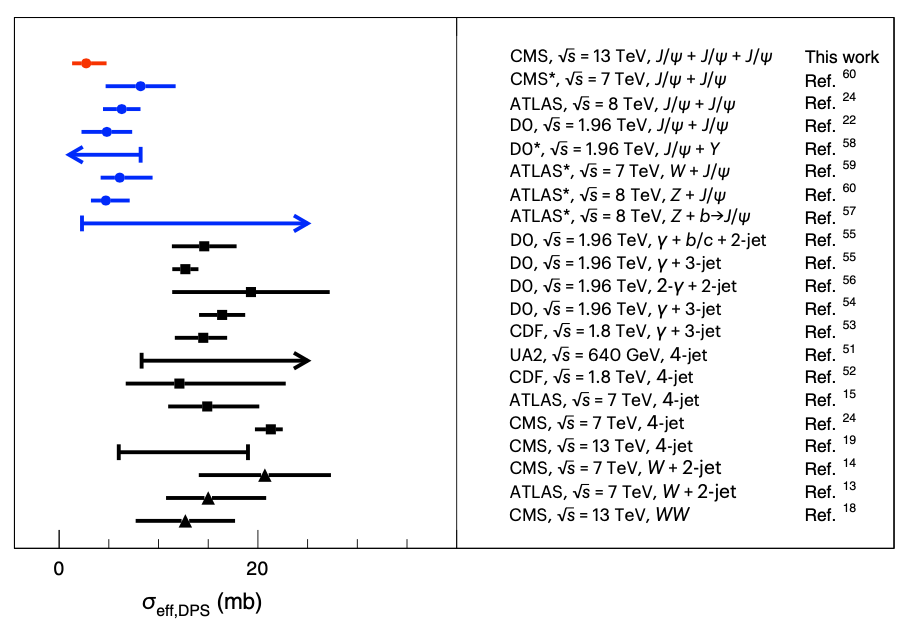
\includegraphics[width=1.0\linewidth]{images/sigma_eff_DPS_summary.png}
    \caption{Summary of current $\effXsecDPS$ measurement results in various final states, including results from the triple-$J/\psi$ production process on the top.\cite{CMS_TRI_JPSI}}
    \label{fig:sigma-eff-dps-summary}
\end{figure}

Disagreement in $\effXsecDPS$ obtained in different methods has been interpreted as from the difference in the dominant parton species probed through such processes \cite{MPI_LHC}, yet in some cases it could also be explained by inadequate SPS component subtraction. Such results calls for independent probes into the proton structure, for instance, triple parton scattering (TPS) processes.

\subsection{Triple Parton Scattering (TPS) Processes}

TPS processes in high-energy proton-proton collisions have drawn much attention both in theory and experiments. In a theoretical work by D. d'Enterria and A. M. Snigirev \cite{DdE_TPS}, it was derived across numerous transverse parton density distributions that, for a DPS processes and a TPS process with similar final states, the effective cross-sections $\effXsecDPS, \effXsecTPS$ satisfy the following relationship:

\begin{equation}
    \label{eqn:dps_tps_eff_xsec}
    \effXsecTPS = \kappa \effXsecDPS \quad (\kappa = 0.82 \pm  0.11)
\end{equation}

A more specific study on TPS processes was conducted by H.-S. Shao and Y.-J. Zhang in 2019\cite{YJZ_TRI_JPSI}, in which they demonstrated the feasibility of using existing data to observe triple-$J/\psi$ hadroproduction and, using this process, to probe into TPS processes. A further work by Y.-J. Zhang demonstrated the feasibility of observing simultaneous production of $J/\psi$, $\Upsilon$ and a $\phi$ meson with $p_T > 2\GeVc$ in high-energy proton-proton collisions\cite{YJZ_MPS_REPORT}.

The triple-$J/\psi$ production in proton-proton collision was soon observed at the CMS experiment, with a DPS effective cross-section of $\effXsecDPS = 2.7^{+1.4}_{-1.0}(\text{exp})^{+1.5}_{-1.0}(\text{theo}) ~\text{mb}$, compatible with previous $\effXsecDPS$ results from di-quarkonia processes. 

Following the pioneering studies in TPS at the CMS experiment, we are motivated to search for simultaneous production of double $J/\psi$ and $\Upsilon$ mesons, double $J/\psi$ and $\phi$ mesons, or $J/\psi$, $\Upsilon$ and $\phi$ mesons in proton-proton collisions at $\sqrt{s} = 13.6 ~ \mathrm{TeV}$ at the CMS experiment. These quarkonia final states have relatively higher cross-sections when compared to jets and electroweak bosons, bringing a larger data sample. It is worth mentioning that, despite a potentially lower yield, the $pp\to J/\psi+J/\psi+\Upsilon+X$ process is included in this analysis, since this process with a 6$\mu$ final state can be more cleanly reconstructed on the CMS detector than the rest of the processes, thanks to the excellent muon identification and measurement capability of the CMS detector. A general introduction is given in the next section.

\subsection{The Large Hadron Collider (LHC)}

The Large Hadron Collider (LHC) operated by the European Organization of Nuclear Research (CERN) is the most powerful accelerator on earth today. The LHC collides beams of protons with an energy of up to 6.8 TeV, corresponding to a center-of-mass energies of up to $\sqrt{s}=13.6~\mathrm{TeV}$. Located approximately 100 meters underground across the Swiss-Franco border near Geneva, the LHC features a main storage ring with a circumference of approximately 27 kilometers, capable of accelerating more than 2800 proton bunches simultaneously, each bunch containing approximately $10^11$ protons. Protons accelerated in the LHC traverse through the storage ring in opposite directions and intersect at four interaction points to collide at a time interval of 25 nanoseconds and deliver an instantaneous luminosity up to $2.5\times 10^{34} ~\text{cm}^{-2}\cdot\text{s}^{-1}$\cite{CMS:LUMI-PUB}.

Four major particle detectors, CMS, ATLAS, ALICE and LHCb, are each located at one of the four interaction points, measuring the key properties of particles produced in collision with their unique detector modules, and acquire data for further physics analysis.

\begin{figure}
    \centering
    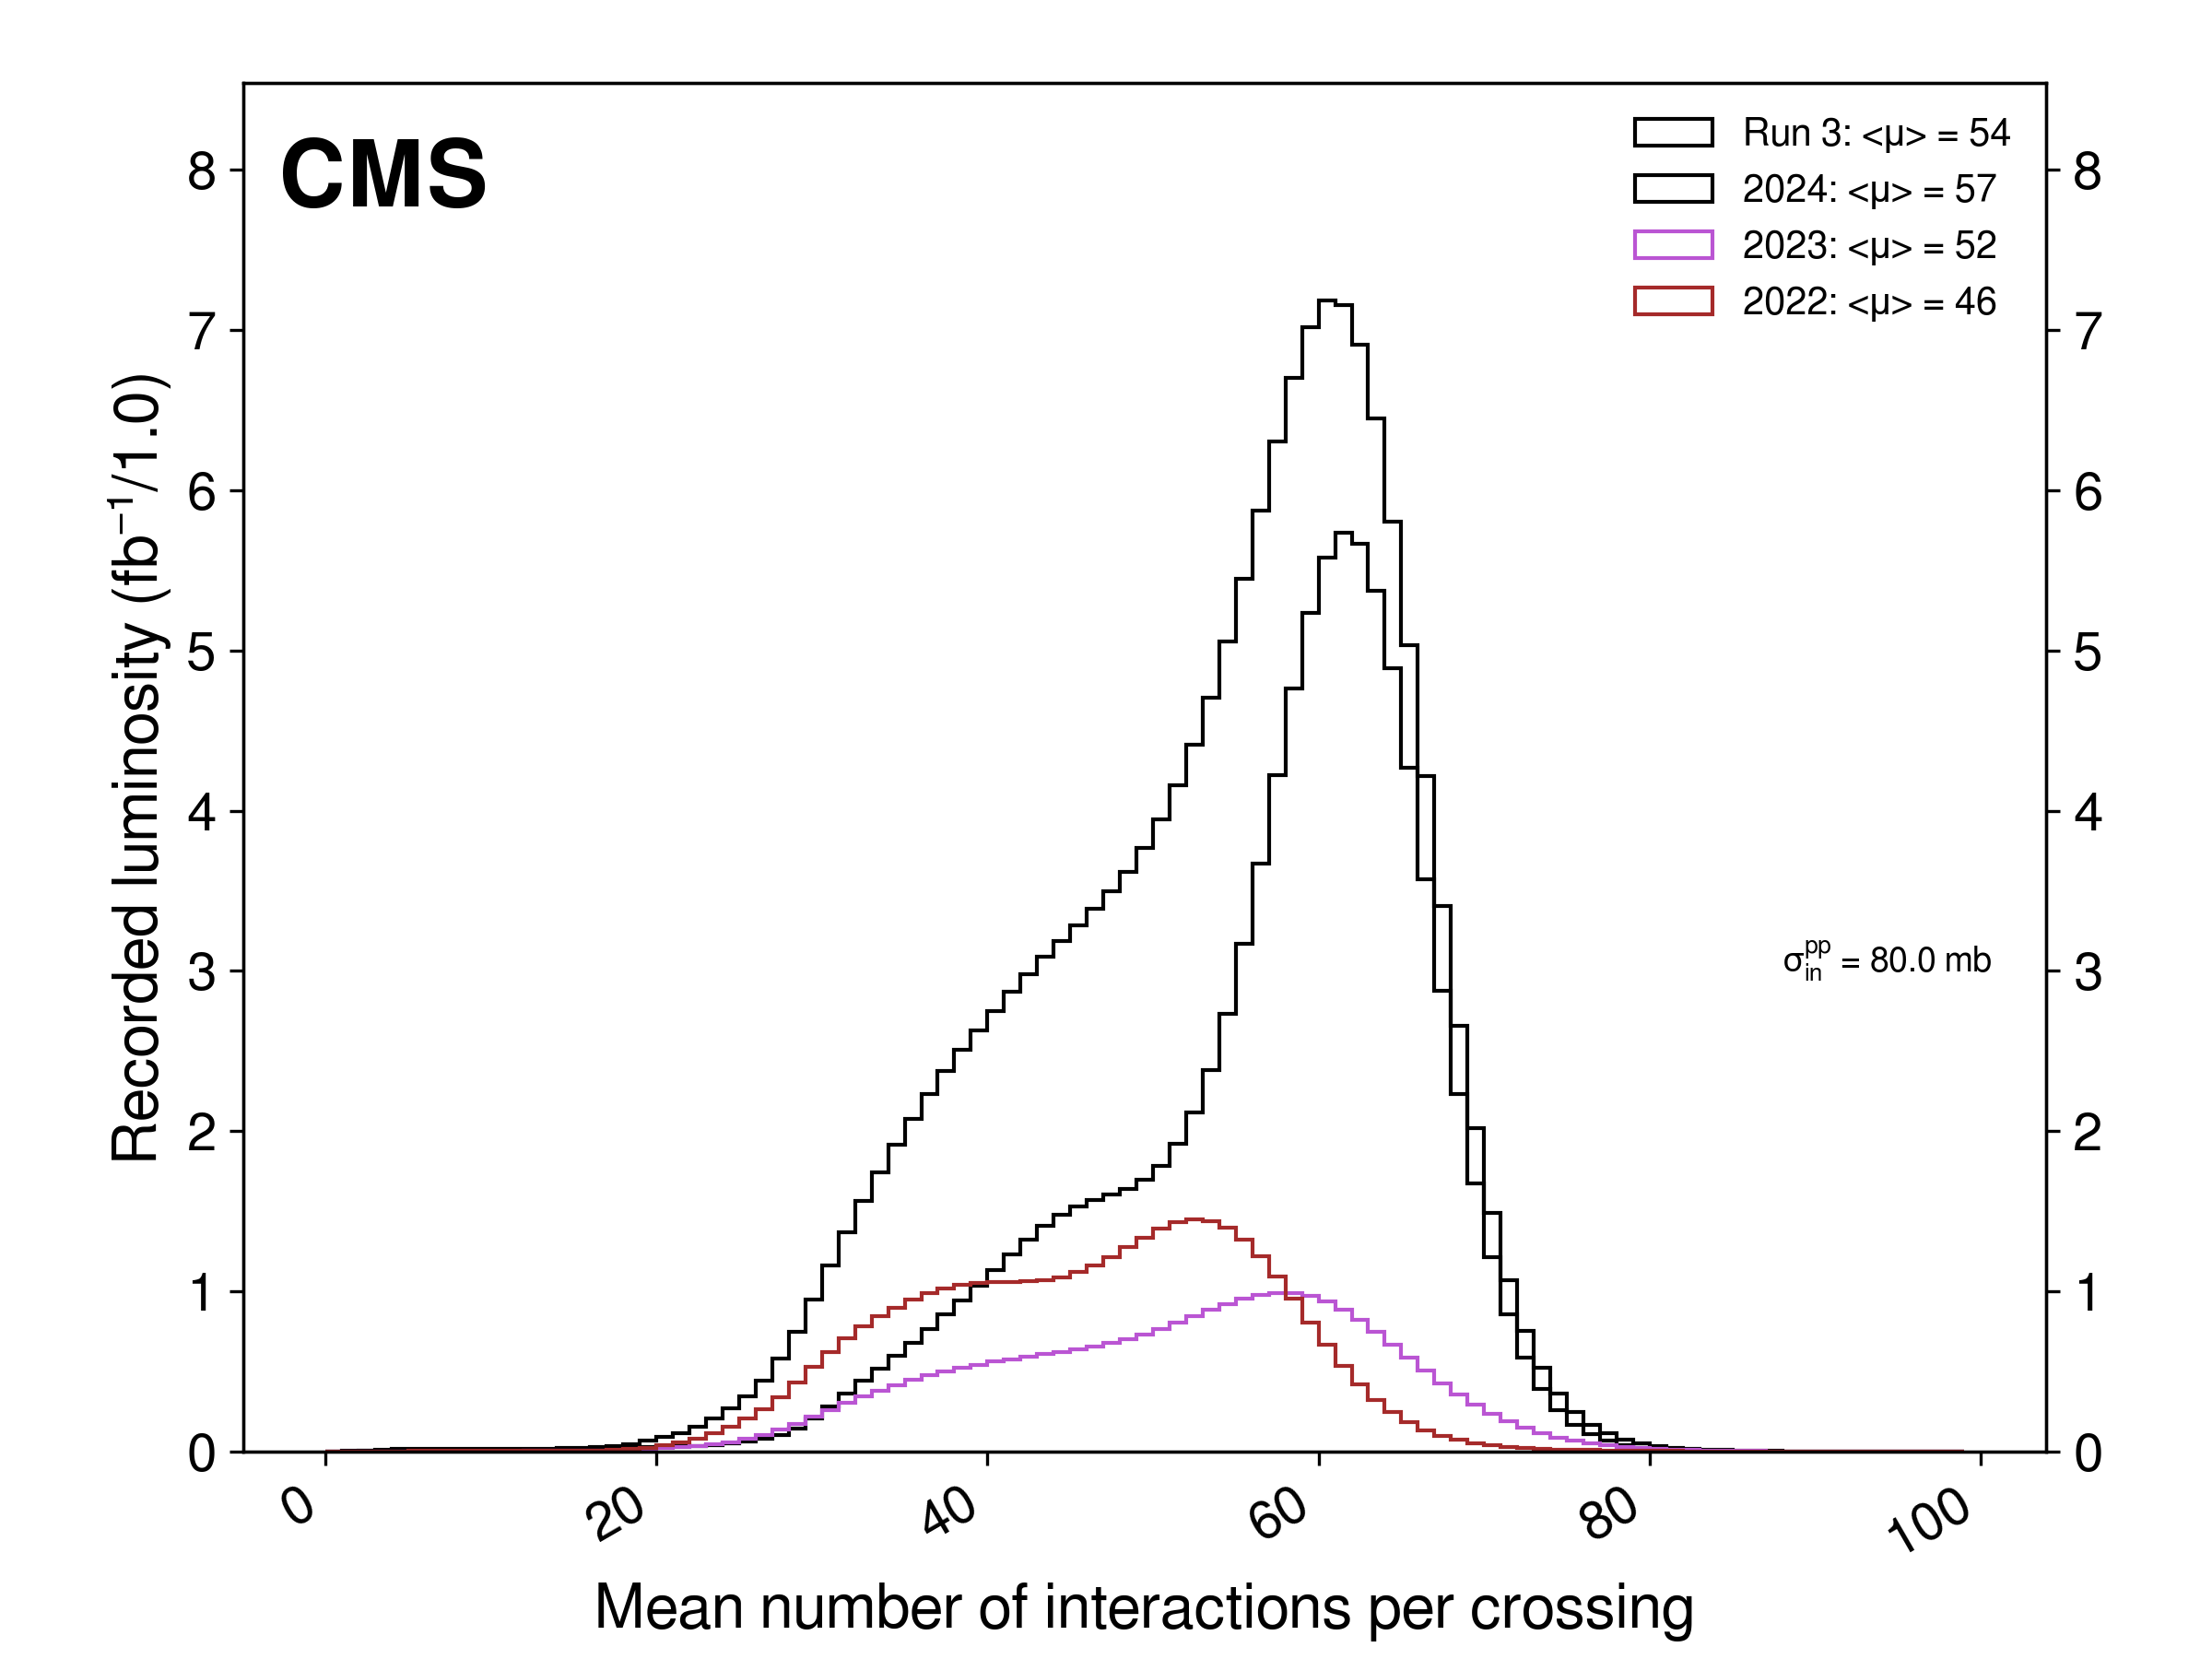
\includegraphics[width=1.0\linewidth]{images/CMS_pileup_allYears_run3.png}
    \caption{Average number of interactions per bunch crossing in LHC Run 3 by year\cite{CMS:LUMI-PUB}}
    \label{fig:CMS_pileup}
\end{figure}

One important consequence of the high luminosity is the "pileup" effect, i.e., in each bunch crossing more than one hard scattering event happens. In LHC Run 3, the average number of interactions in each bunch crossing reaches 60, as shown by Figure \ref{fig:CMS_pileup}. \cite{CMS:LUMI-PUB} Such effect may introduce a higher combinatorial background in the analysis and require advanced analysis techniques to mitigate its effect.

\subsection{The CMS Detector}

The Compact Muon Solenoid (CMS) (shown in Figure \ref{fig:CMS-disection}) is one of the two general-purpose detectors on LHC. The detector itself measures 21 meters long and 15 meters in diameter, with a total weight of approximately 14,000 tonnes.

\begin{figure}
    \centering
    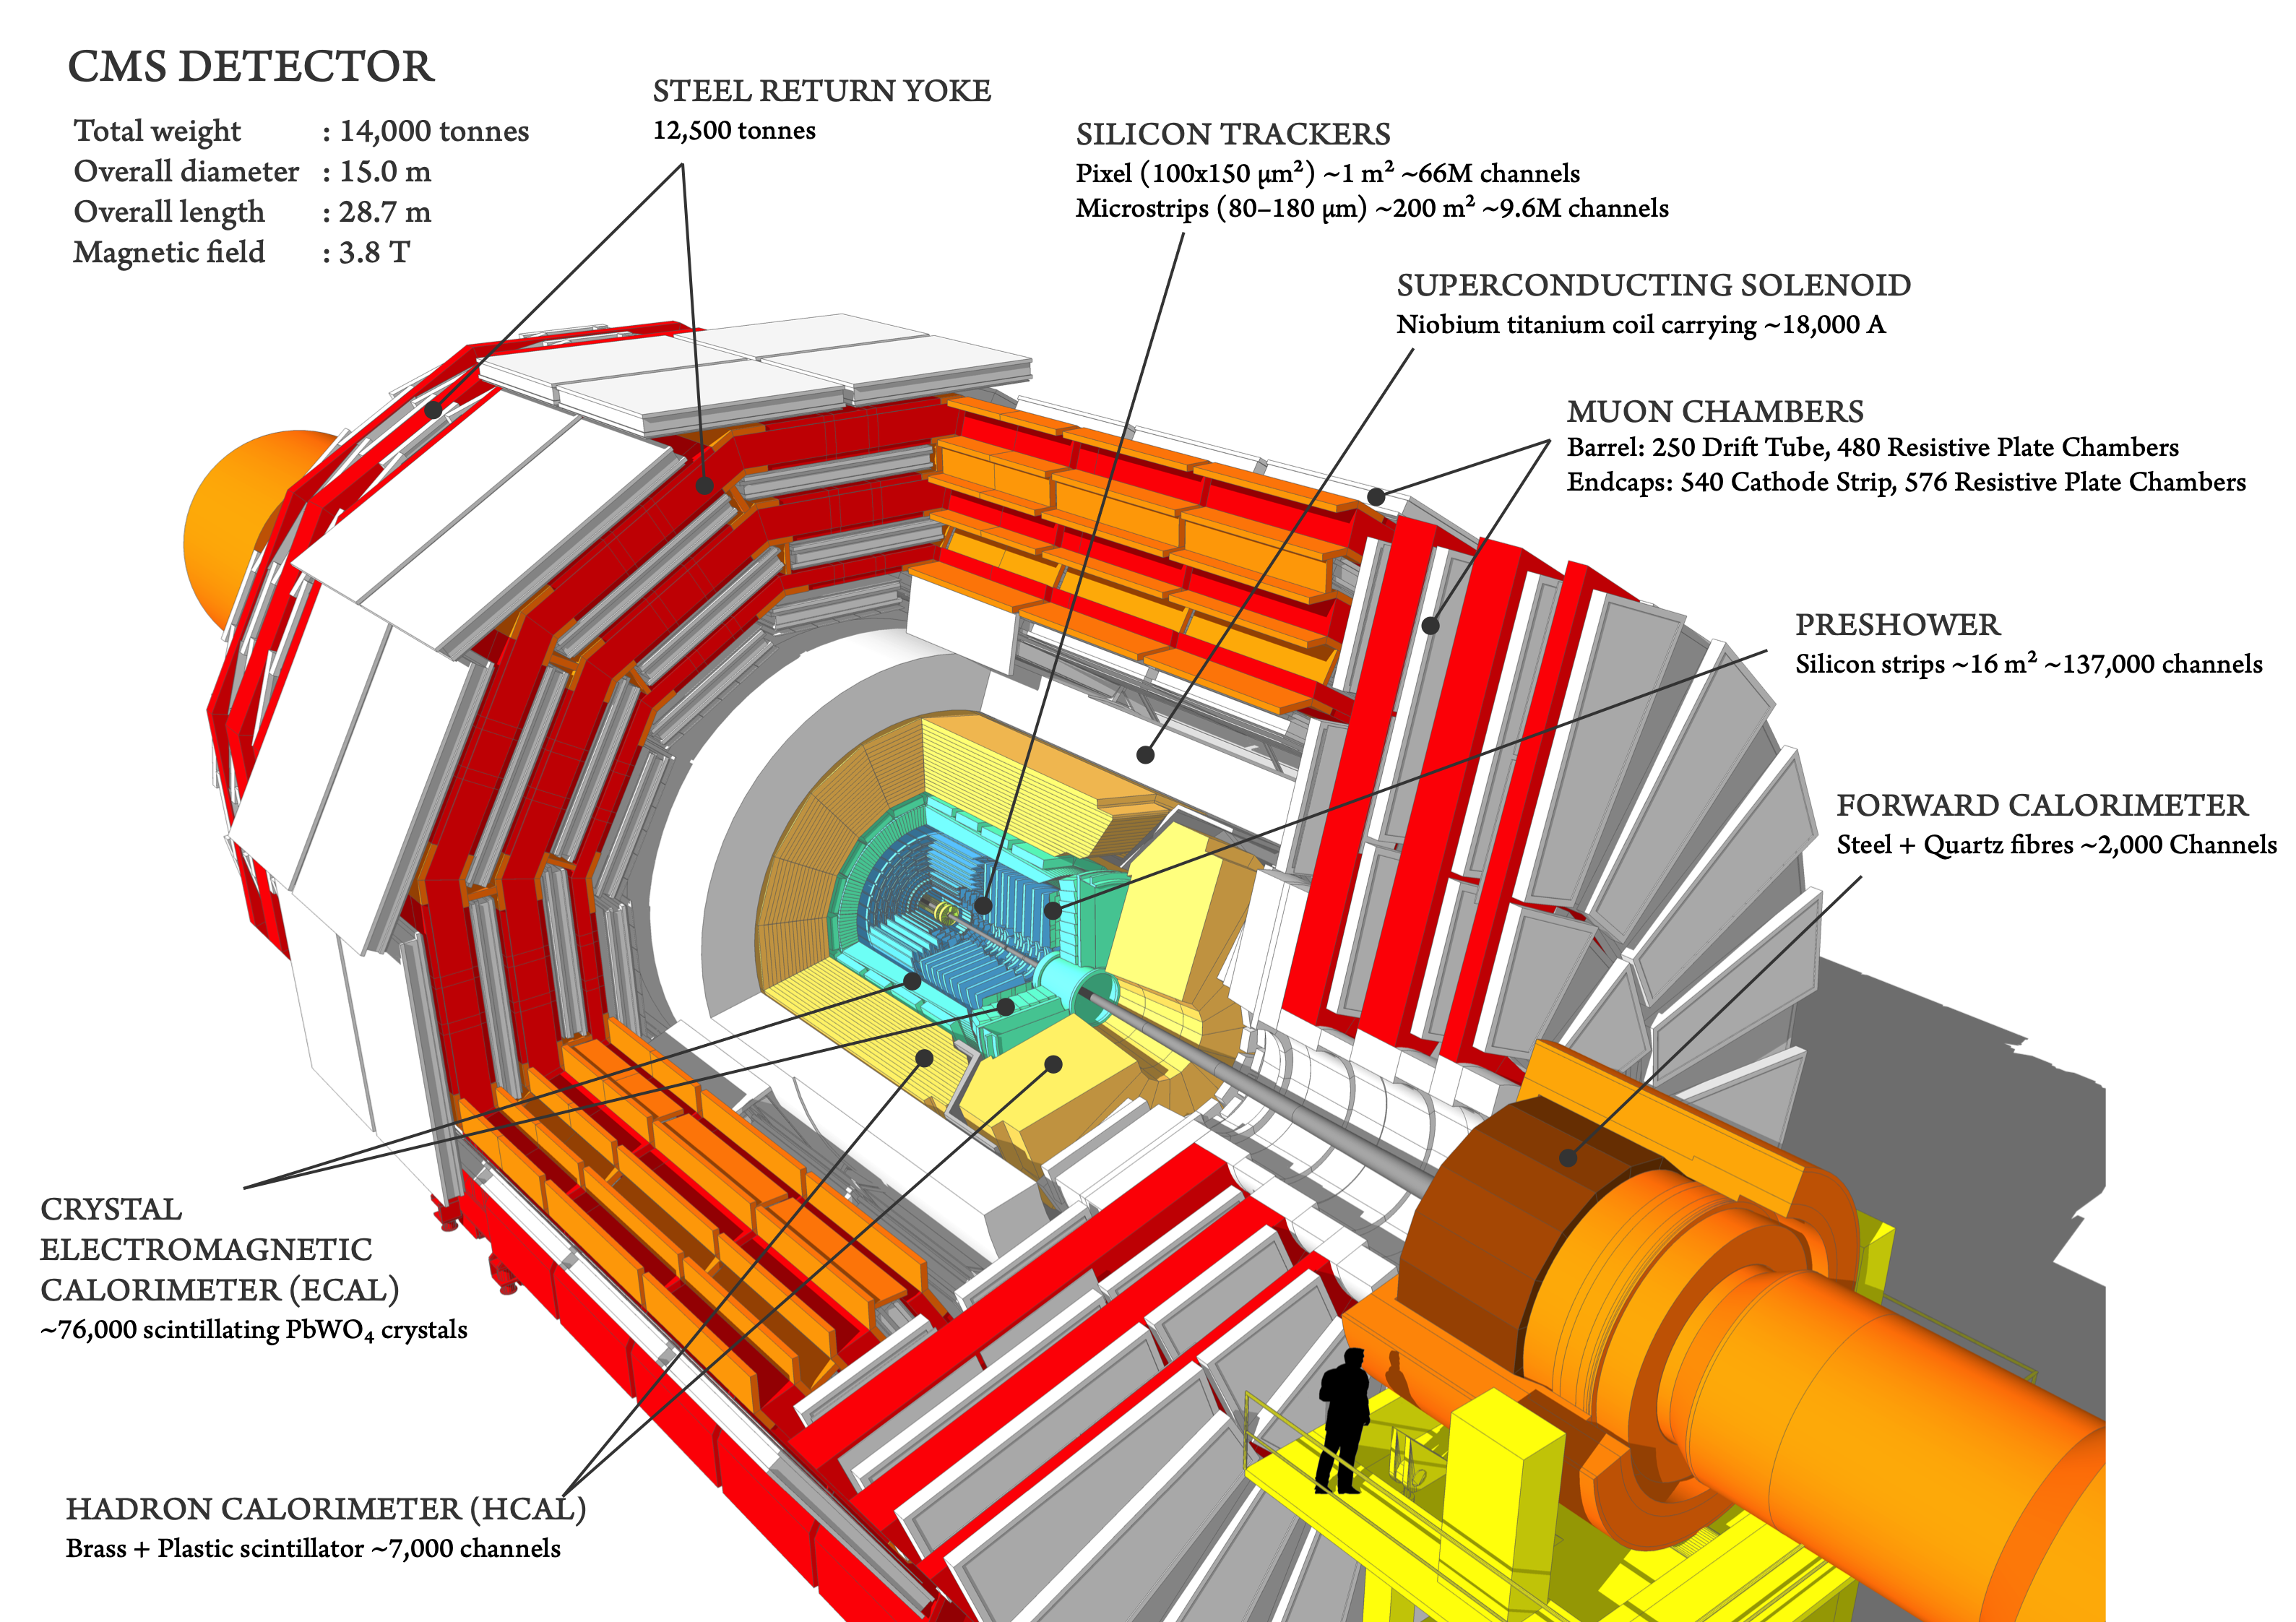
\includegraphics[width=1.0\linewidth]{images/CMS_disection_Run2.png}
    \caption{A schematic dissection of the CMS detector\cite{CMS_CUTAWAY_DIAGRAM}}
    \label{fig:CMS-disection}
\end{figure}

A defining characteristic of CMS is its powerful superconducting solenoid magnet with a inner bore of 5.9 meters and a length of 12.9 meters, capable of producing a magnetic field of 3.8 T inside its bore with a direction along the beam line, where the inner tracker and calorimeter modules are accommodated. The strong-magnetic-field design is in line with the demand for good momentum resolution within a relatively compact spectrometer.\cite{CMS_JINST_2008}

Another distinctive advantage of CMS is its muon measurement capability, owing to its muon sub-detector module designs. With the return field of the superconducting solenoid strong enough to saturate 1.5 m of iron, the 4 muon "stations" are integrated inside the iron return yoke of the solenoid, providing a bending field of around 2 T and ensuring both robustness and full geometrical coverage. Each muon "station" consists of several layers of aluminium drift tubes (DT) in the barrel region and and cathode strip chambers (CSCs) in the endcap region, complemented by resistive plate chambers (RPCs). These detector modules work in tandem with the inner silicon tracker modules to produce a total reconstruction and identificaton efficiency of $> ~ 96\%$ and relative momentum resolution of $2\%$ for most muons and $10\%$ even for TeV muons.\cite{CMS_MUON_PERF_13TEV}

\section{Datasets and Event Selection}

\subsection{Dataset}

The datasets analyzed are \textsc{ParkingDoubleMuonLowMass} collected from 2022 to 2024, entirely during the LHC Run 3 period with a collision energy of $\sqrt{s} = 13.6 ~\text{TeV}$ and an integrated luminosity of $\mathcal{L}\approx176.6~\text{fb}^{-1}$. The datasets are required to be certified as "muon" physics datasets.\cite{CMS:LUM-22-001}\cite{CMS:DP-LUMI-2023}\cite{CMS:LUMI-PUB}.

% \begin{figure}
%     \centering
%     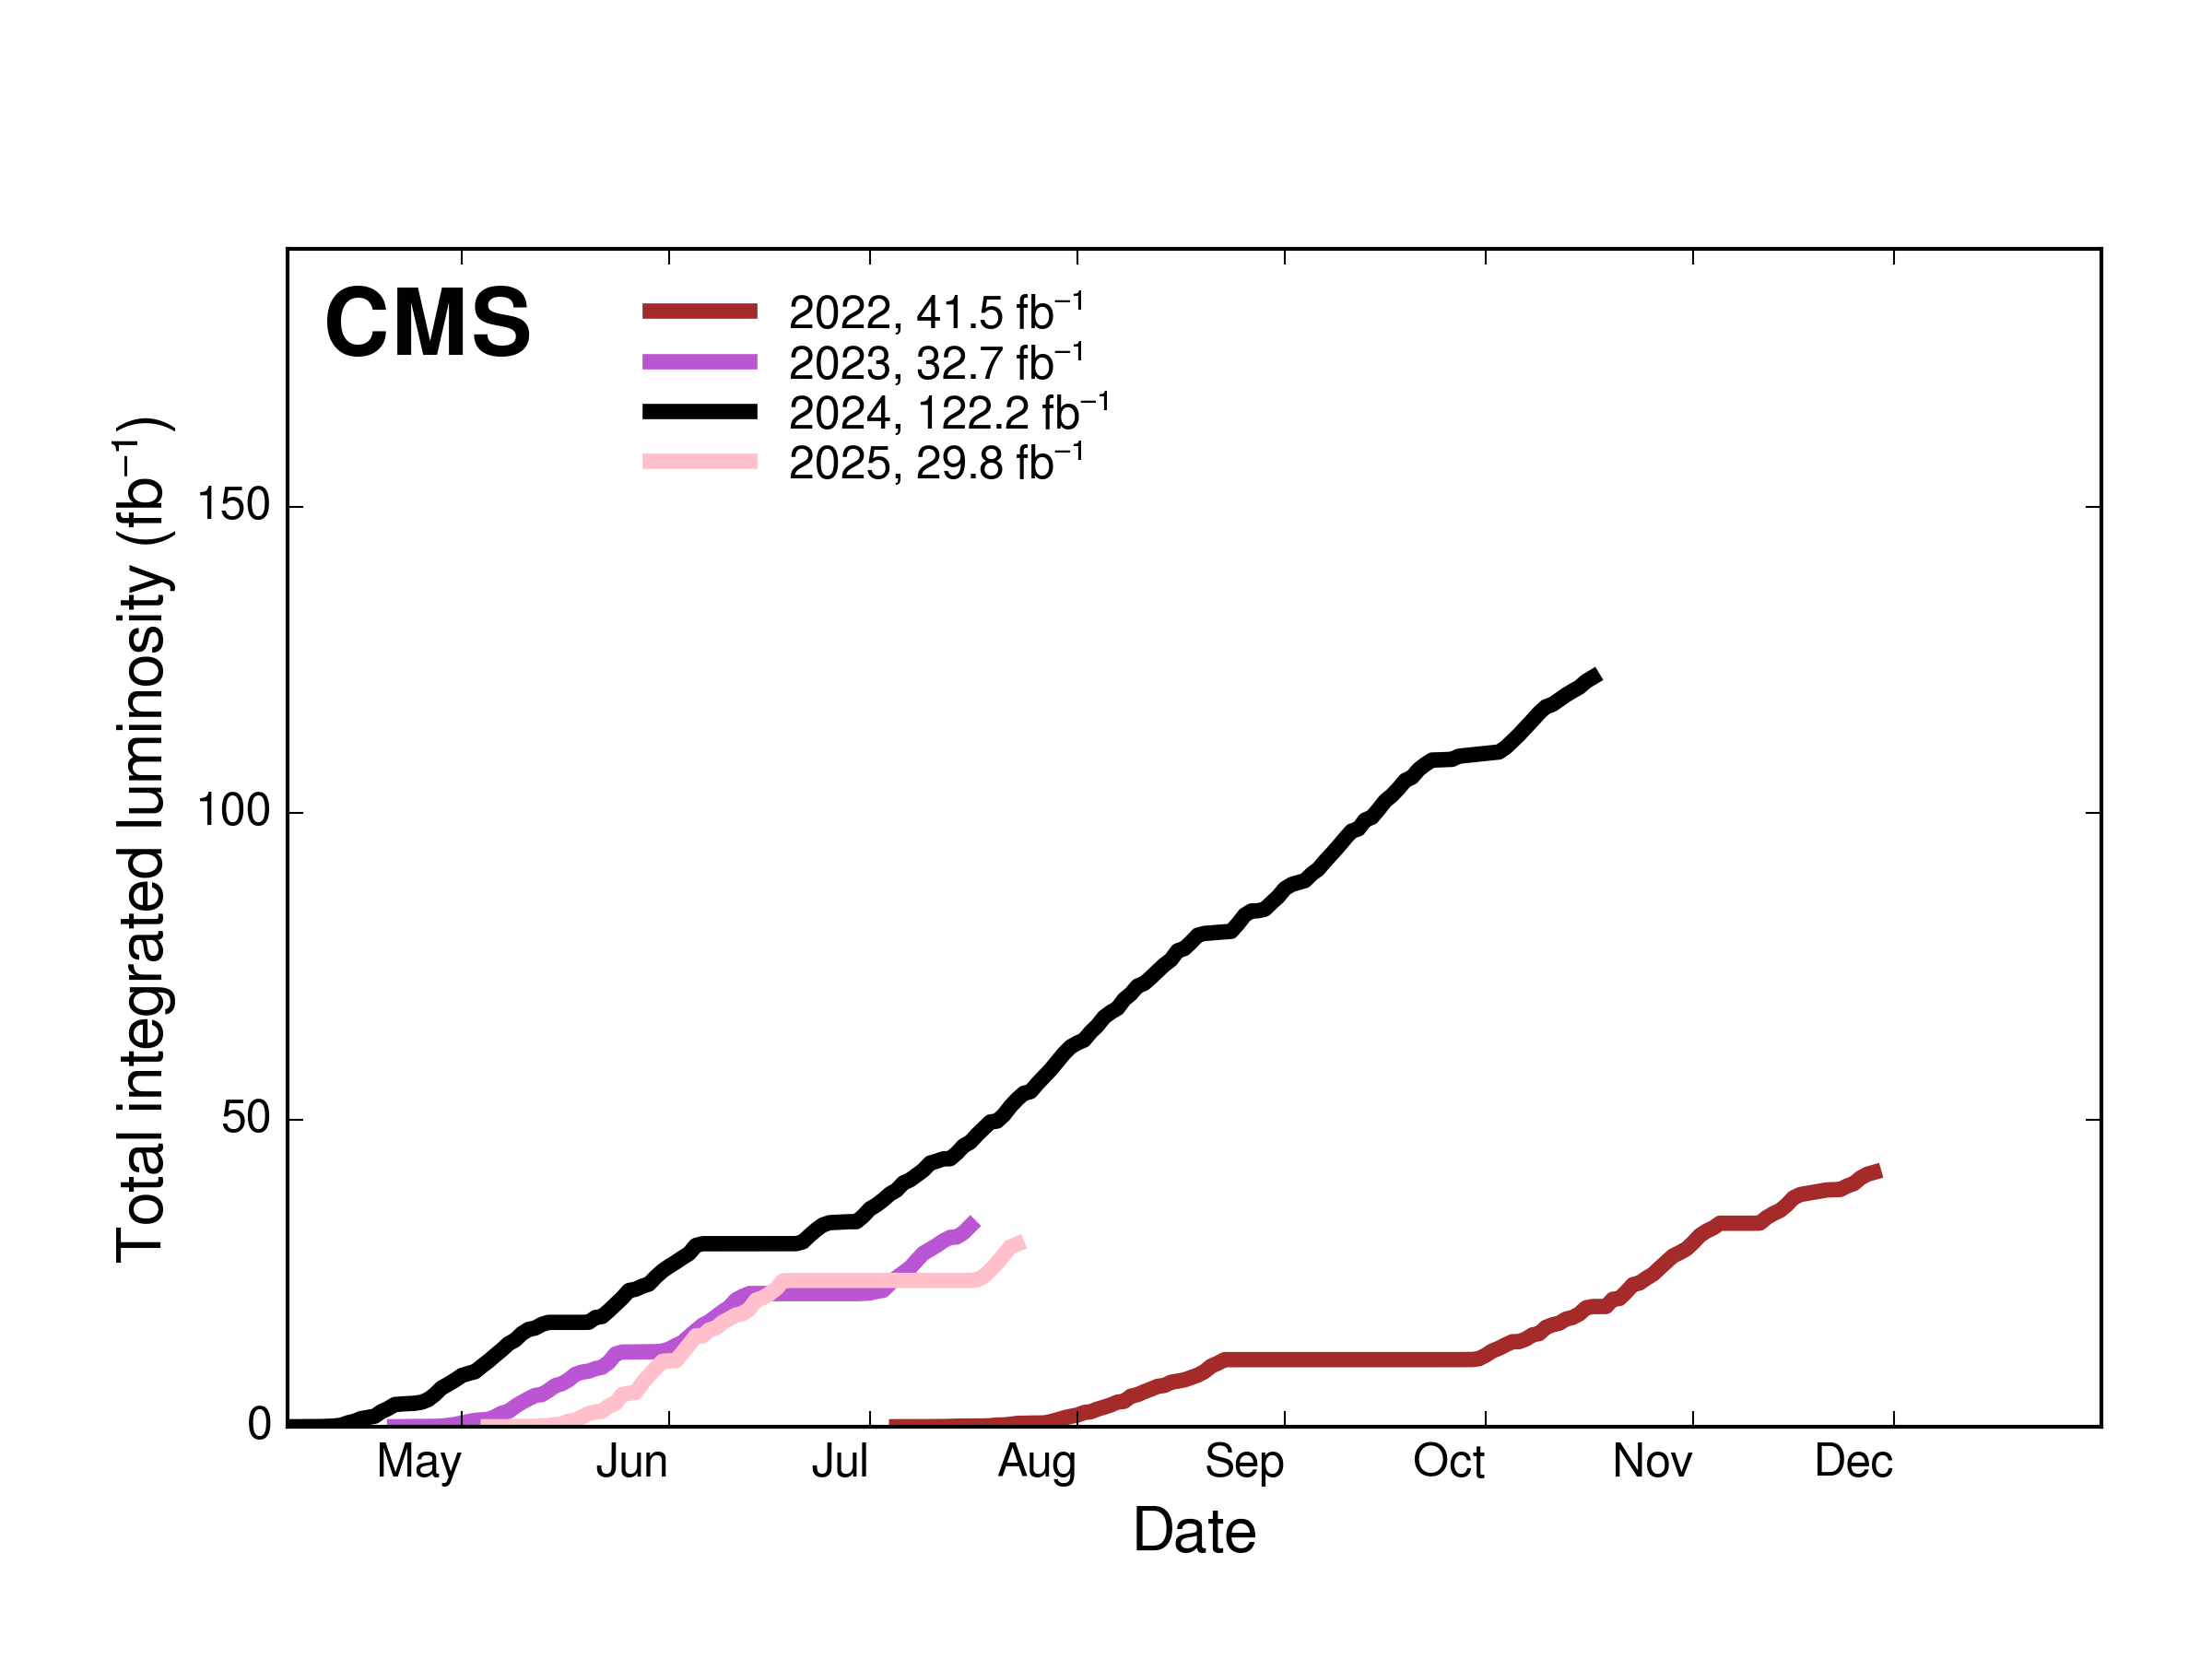
\includegraphics[width=1.0\linewidth]{images/CMS_int_lumi_Run3.png}
%     \caption{Cumulative luminosity delivered to CMS versus date during  LHC Run 3 \cite{CMS:LUMI-PUB}}
%     \label{fig:CMS_int_lumi}
% \end{figure}

\begin{table*}[h!]
    \centering
    \caption{Datasets and corresponding JSON files analyzed\\}
    \label{tab:dataset}
    \begin{tabular}{c}
    \toprule
     \multicolumn{1}{l}{\textbf{2022} - Cert\_Collisions2022\_355100\_362760\_Muon.json}\\
     ParkingDoubleMuonLowMass[0-7]/Run2022C-PromptReco-v1/MINIAOD\\
     ParkingDoubleMuonLowMass[0-7]/Run2022D-PromptReco-v1/MINIAOD\\
     ParkingDoubleMuonLowMass[0-7]/Run2022D-PromptReco-v2/MINIAOD\\
     ParkingDoubleMuonLowMass[0-7]/Run2022E-PromptReco-v1/MINIAOD\\
     ParkingDoubleMuonLowMass[0-7]/Run2022F-PromptReco-v1/MINIAOD\\
     ParkingDoubleMuonLowMass[0-7]/Run2022G-PromptReco-v1/MINIAOD\\
     \midrule
     \multicolumn{1}{l}{\textbf{2023} - Cert\_Collisions2023\_366442\_370790\_Muon.json}\\
     ParkingDoubleMuonLowMass[0-7]/Run2023C-PromptReco-v1/MINIAOD\\
     ParkingDoubleMuonLowMass[0-7]/Run2023C-PromptReco-v2/MINIAOD\\
     ParkingDoubleMuonLowMass[0-7]/Run2023C-PromptReco-v3/MINIAOD\\
     ParkingDoubleMuonLowMass[0-7]/Run2023C-PromptReco-v4/MINIAOD\\
     ParkingDoubleMuonLowMass[0-7]/Run2023D-PromptReco-v1/MINIAOD\\
     ParkingDoubleMuonLowMass[0-7]/Run2023D-PromptReco-v2/MINIAOD\\
     \midrule
     \multicolumn{1}{l}{\textbf{2024} - Cert\_Collisions2024\_378981\_386951\_Muon.json}\\
     ParkingDoubleMuonLowMass[0-7]/Run2024C-PromptReco-v1/MINIAOD\\
     ParkingDoubleMuonLowMass[0-7]/Run2024D-PromptReco-v1/MINIAOD\\
     ParkingDoubleMuonLowMass[0-7]/Run2024E-PromptReco-v1/MINIAOD\\
     ParkingDoubleMuonLowMass[0-7]/Run2024E-PromptReco-v2/MINIAOD\\
     ParkingDoubleMuonLowMass[0-7]/Run2024F-PromptReco-v1/MINIAOD\\
     ParkingDoubleMuonLowMass[0-7]/Run2024G-PromptReco-v1/MINIAOD\\
     ParkingDoubleMuonLowMass[0-7]/Run2024H-PromptReco-v1/MINIAOD\\
     ParkingDoubleMuonLowMass[0-7]/Run2024I-PromptReco-v1/MINIAOD\\
     ParkingDoubleMuonLowMass[0-7]/Run2024I-PromptReco-v2/MINIAOD\\
     \bottomrule
    \end{tabular}
\end{table*}

\subsection{The CMS Trigger System and Criteria}

LHC collisions occur at a rate of 40 MHz, which corresponds to a data production rate of around 40 TB/s, making it impossible to store all events. The CMS experiment therfore employs a a two-tiered trigger system to preserve only events of physical importance. A hardware-based Level 1 Trigger (L1T), run on FPGAs and ASICs, reduces the event rate to 100 kHz. A software-based High Level Trigger (HLT), run on computer farms further reduces the average output rate to around 1.5 kHz.

The CMS datasets typically accept events passing any one of a certain set of trigger conditions. In our analysis, we require the events to be triggered by the \textsc{HLT\_Dimuon0\_Jpsi3p5\_Muon2\_v} or the \textsc{HLT\_Trimuon5\_3p5\_2\_Upsilon\_Muon\_v}, with the primary criteria of each trigger listed in Table \ref{tab:trigger}. The former trigger is used to extract potential $J/\psi\to\mu^+\mu^-$ processes and the latter one is used to obtain more $\Upsilon(nS)$-containing samples.

\begin{table*}[ht]
    \centering
    \caption{Primary selection criteria of the triggers employed}
    \begin{tabular}{p{0.45\textwidth}p{0.45\textwidth}}
    \toprule
    \textbf{HLT\_Dimuon0\_Jpsi3p5\_Muon2\_v}  &
    \textbf{HLT\_Trimuon5\_3p5\_2\_Upsilon\_Muon\_v} \\
    \midrule
    At least 3 muons present and satisfying: &
    At least 3 muons present and satisfying: \\
    \begin{itemize}[topsep=0pt, leftmargin=*]
        \item Transverse momentum $p_T > 2.0\GeVc$
        \item Pseudorapidity $|\eta| < 2.5$
    \end{itemize} &
    \begin{itemize}[topsep=0pt, leftmargin=*]
        \item Transverse momentum $p_T > 2.0\GeVc$
        \item Pseudorapidity $|\eta| < 2.5$
    \end{itemize}\\
    & $\mathbf{\cdot}$ At least 1 muon satisfying $p_T > 5.0 \GeVc$ \\
    \midrule
    With at least one pair of muon satisfying : &
    With at least one pair of muon satisfying : \\
    \begin{itemize}[topsep=0pt, leftmargin=*]
        \item $p_T > 3.5\GeVc$
        \item Invariant mass $m_{\mu\mu}$ satisfying $2.95\GeVcs < m_{\mu\mu} < 3.25 \GeVcs$
        \item Tracks fitted to a common vertex with probability > $0.5\%$
    \end{itemize} &
    \begin{itemize}[topsep=0pt, leftmargin=*]
        \item $p_T > 3.5\GeVc$
        \item Invariant mass $m_{\mu\mu}$ satisfying $8.5\GeVcs < m_{\mu\mu} < 11.4 \GeVcs$
        \item Tracks fitted to a common vertex with probability > $0.5\%$
    \end{itemize} \\
    \bottomrule
    \end{tabular}

    \label{tab:trigger}
\end{table*}

\subsection{Final State Particle Selection}

Given the excellent muon identification and measurement capability of the CMS detector,  we choose $J/\psi\to\mu^+\mu^-$ and $\Upsilon(nS)\to\mu^+\mu^-$ as the decay channel of these two heavy quarkonia. For $\phi$ mesons, the decay channel $\phi\to K^+K^-$ is chosen due to a relatively large branching ratio ($\approx 49\%$) \cite{PDG2020}.

In reconstruction of $\phi$ mesons, due to a relatively low identification ability for soft charged particles, all non-muon charged tracks are assumed to be $K^\pm $ and the tracks are paired only with the opposite-sign requirement.

Given that the transverse momenta of these final-state paticles typically fall in the $\text{GeV}$ region, the dominant background component for simultaneous production is the combinatorial background, with uncorrelated muons from semileptonic decay of beauty- and charm-quark hadron decays and Drell Yan events forming background in $m_{\mu\mu}$ spectra, and other charged particles from soft-QCD processes forming background in the $m_{KK}$ spectrum\cite{CMS_TRI_JPSI}.

To reduce background components, a further set of selection is applied to the objects for event reconstruction and signal extraction, as will be discussed in the next section.

\section{Signal Extraction}

\subsection{Data Analysis for $pp\to J/\psi+J/\psi+\phi+X$}

In extracting $pp\to J/\psi+J/\psi+\phi+X$ signals, we require further conditions shown in Table \ref{tab:cut_JpsiJpsiPhi} for the reconstructed candidate event, in which the pseudorapidity $y$ is defined by (where direction $z$ is taken to be the beam direction):

\begin{equation}
    y = \frac{1}{2} \ln \frac {E-p_z}{E+p_z}
\end{equation}

The transverse momentum $p_T$ is defined as:

\begin{equation}
    p_T = \sqrt{p_x^2 + p_y^2}
\end{equation}

The pseudorapidity $\eta$ is defined as:

\begin{equation}
    \eta = -\ln \tan \frac{\theta}{2}
\end{equation}

where the polar angle $\theta$ is defined as the angle between the particle momentum vector and the beam direction.

It is worth mentioning that the $p_T > 4.0\GeVc$ selection for $\phi$ meson is also necessary to warranty true hard-scattering processes, since $\phi(s\bar{s})$ is a light flavour meson and can be produced in large amounts in soft-QCD processes in the collision with $p_T\lesssim 1\GeVc$. A proper $p_T$ threshold can effectively remove contribution from such soft processes.

\begin{table}[]
    \centering
    \caption{Event selection for $pp\to J/\psi+J/\psi+\phi+X$ candidate events\\}
    \begin{tabular}{c p{0.66\linewidth}}
        \toprule
        \textbf{Object} & \textbf{Criteria} \\
        \midrule
        $\mu^\pm $ & Muon ID "soft" \\
                  & $|\eta| < 2.4$ \\
                  & $p_T > 3.5\GeVc$ for $|\eta| < 1.2$ \\
                  & $p_T > 2.5\GeVc$ for $1.2 < |\eta| < 2.4$ \\
                  \midrule
        Charged Tracks & High Purity \\
                  & $|\eta|<2.5$ \\
                  & $p_T > 2.0 \GeVc$ \\
        \midrule
        $J/\psi$ & $2.9 \GeVcs < m_{\mu\mu} < 3.3 \GeVcs$ \\
                 & $p_T > 6.0\GeVc$ \\
                 & $|y| < 2.5$ \\
                 & Opposite-sign muon pairs fitted to common vertex with $> 1\%$ probability \\
                 \midrule
        $J/\psi+J/\psi$ & Two $J/\psi$ candidates fitted to a common vertex with $> 1\%$ probability \\
        \midrule
        $\phi$ & $0.99 \GeVcs < m_{KK} < 1.07 \GeVcs$ \\
               & Opposite-sign non-muon charged tracks fitted to common vertex with $> 1\%$ probability \\
               & $p_T > 4.0\GeVc$ \\
               \midrule
        $J/\psi+J/\psi+\phi$ & Three mesons fitted to a common vertex with "valid" result \\
        \bottomrule
    \end{tabular}
    \label{tab:cut_JpsiJpsiPhi}
\end{table}

A three-dimensional maximum likelihood fit is used to extract the signal components. The $J/\psi$ signal shape is modelled with the sum of a Crystal Ball function and a Gaussian function, with all parameters left to float and background modelled by an exponential function. The $\phi$ signal shape on the di-Kaon invariant mass spectrum is taken to be a Gaussian function, also with all parameters left free to float and its combinatorial background modelled by a 4th-order polynomial. With all signal and backround components, we define further eight yield parameters.

\begin{figure}
    \centering
    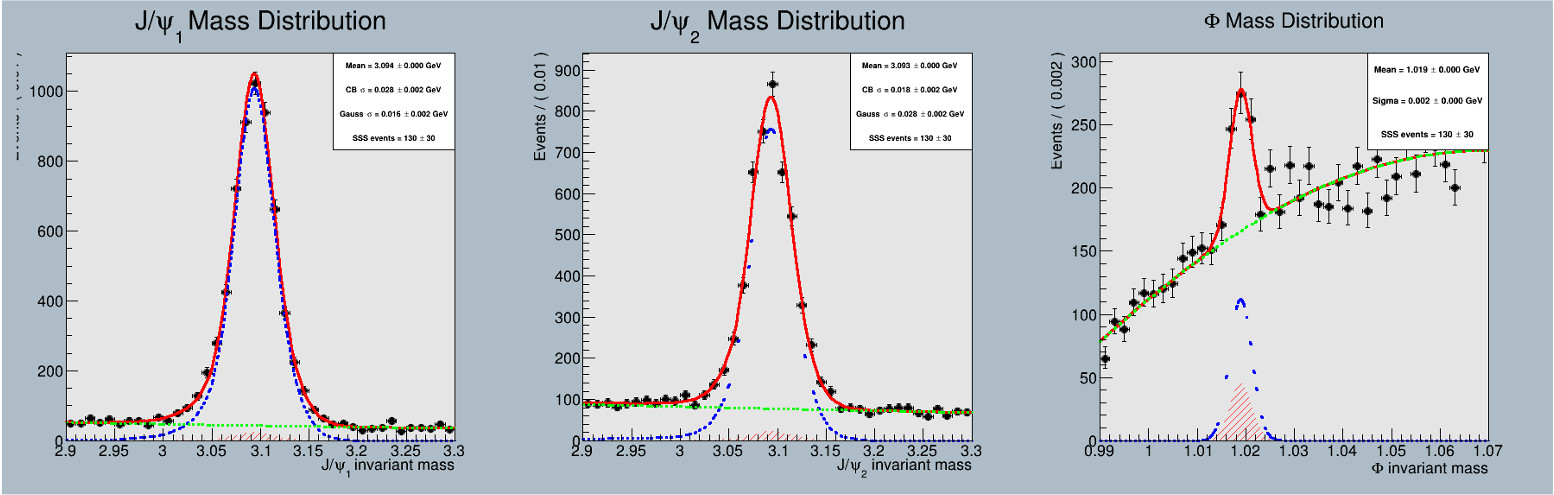
\includegraphics[width=1.0\linewidth]{images/JpsiJpsiPhi_fit.png}
    \caption{Fit result projection on individual invariant mass spectra}
    \label{fig:JpsiJpsiPhi_fit}
\end{figure}

The fit result projection is shown in Figure  \ref{fig:JpsiJpsiPhi_fit}, with $130 \pm 30$ events seen from approximately 7450 candidate events.

\begin{table}[]
    \centering
    \caption{}
    \begin{tabular}{cc}
        \toprule
        \textbf{Yield Parameter} & \textbf{Value} \\
        \midrule
        $N(J/\psi^{[1], \text{sig} },J/\psi^{[2],\text{sig} }, \phi^\text{sig})$ & $130 \pm 30$ \\
        $N(J/\psi^{[1], \text{bkg} },J/\psi^{[2],\text{sig} }, \phi^\text{sig})$ & $52 \pm 18$ \\
        $N(J/\psi^{[1], \text{sig} },J/\psi^{[2],\text{bkg} }, \phi^\text{sig})$ & $90 \pm 27$ \\
        $N(J/\psi^{[1], \text{sig} },J/\psi^{[2],\text{sig} }, \phi^\text{bkg})$ & $3476 \pm 128$ \\
        $N(J/\psi^{[1], \text{bkg} },J/\psi^{[2],\text{bkg} }, \phi^\text{sig})$ & $48 \pm 19$ \\
        $N(J/\psi^{[1], \text{bkg} },J/\psi^{[2],\text{sig} }, \phi^\text{bkg})$ & $684 \pm 55$ \\
        $N(J/\psi^{[1], \text{sig} },J/\psi^{[2],\text{bkg} }, \phi^\text{bkg})$ & $2024 \pm 120$ \\
        $N(J/\psi^{[1], \text{bkg} },J/\psi^{[2],\text{bkg} }, \phi^\text{bkg})$ & $943 \pm 54$ \\
        \bottomrule
    \end{tabular}
    \label{tab:fitres_JpsiJpsiPhi}
\end{table}

The yield parameters obtained through fitting are as listed in Table \ref{tab:fitres_JpsiJpsiPhi}. The predominant background seen from fitting is double-$J/\psi$ events without $\phi$ mesons, and a signal significance of $4.7 \sigma$ is concluded for the simultaneous production. The efficiency and cross-section analysis are to be determined with further Monte Carlo analyses.

\subsection{Data Analysis for $pp\to J/\psi+\Upsilon+\phi+X$}

In extracting $pp\to J/\psi+\Upsilon+\phi+X$ signals, a set of selection criteria is shown in Table \ref{tab:cut_JpsiYPhi} for the reconstructed candidate event. Compared to the criteria required for $pp \to J/\psi+J/\psi+\phi+X$ analysis, a lower cross section is expected from the relatively low yield of $\Upsilon$ compared to $J/\psi$. The $p_T$ threshold for $J/\psi$ and $\phi$ is thus lowered to enable more candidate events to pass the selection. In the lower-$p_T$ region, however, a higher combinatorial background can be seen and, to compensate for this, the threshold for $J/\psi$ and $\phi$ decay vertex fit probabilities is increased to further reject backgrounds.

\begin{table}[]
    \centering
    \caption{Event selection for $pp\to J/\psi+\Upsilon+\phi+X$ candidate events\\}
    \begin{tabular}{c p{0.66\linewidth}}
        \toprule
        \textbf{Object} & \textbf{Criteria} \\
        \midrule
        $\mu^\pm $ & Muon ID "soft" \\
                  & $|\eta| < 2.4$ \\
                  & $p_T > 3.5\GeVc$ for $|\eta| < 1.2$ \\
                  & $p_T > 2.5\GeVc$ for $1.2 < |\eta| < 2.4$ \\
                  \midrule
        Charged Tracks & High Purity \\
                  & $|\eta|<2.5$ \\
                  & $p_T > 2.0 \GeVc$ \\
        \midrule
        $J/\psi$ & $2.9 \GeVcs < m_{\mu\mu} < 3.3 \GeVcs$ \\
                 & $p_T > 4.0\GeVc$ \\
                 & $|y| < 2.5$ \\
                 & Opposite-sign muon pairs fitted to common vertex with $> 5\%$ probability \\
                 \midrule
        $\Upsilon$ & $8.5\GeVcs < m_{\mu\mu} < 11.4 \GeVcs$ \\
                 & $p_T > 4.0\GeVc$ \\
                 & $|y| < 2.5$ \\
                 & Opposite-sign muon pairs fitted to common vertex with $> 5\%$ probability \\
                 & Reconstructed from muons passing "Tight" muon ID \\
                 \midrule
        $J/\psi+\Upsilon$ & Two candidates fitted to a common vertex with $> 1\%$ probability \\
        \midrule
        $\phi$ & $0.99 \GeVcs < m_{KK} < 1.07 \GeVcs$ \\
               & Opposite-sign non-muon charged tracks fitted to common vertex with $> 5\%$ probability \\
               & $p_T > 2.0\GeVc$ \\
               \midrule
        $J/\psi+J/\psi+\phi$ & Three mesons fitted to a common vertex with "valid" result \\
        \bottomrule
    \end{tabular}
    \label{tab:cut_JpsiYPhi}
\end{table}

A three-dimensional maximum likelihood fit is used to extract the signal components, with similar $J/\psi$ and $\phi$ signal shapes and each $\Upsilon$ resonance modelled by the sum of two CB functions, keeping only $\Upsilon(1S)$ mass and the fraction between the yields of different resonances to float.

\begin{figure}
    \centering
    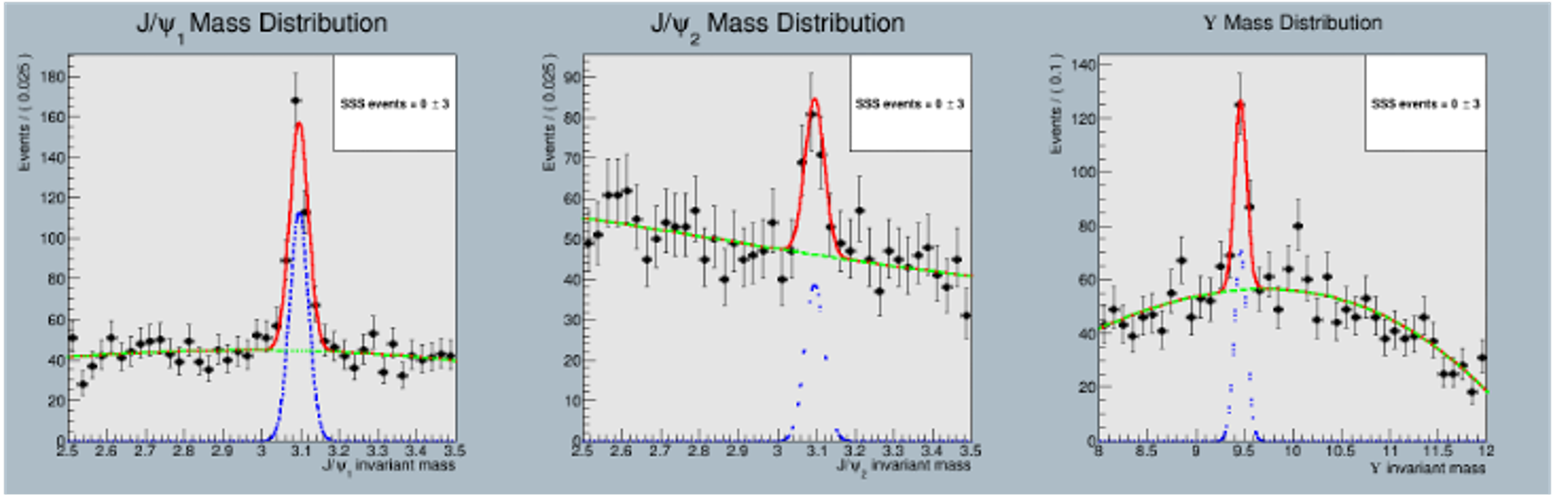
\includegraphics[width=1.0\linewidth]{images/JpsiJpsiY_fit.png}
    \caption{Fit result projection on individual invariant mass spectra}
    \label{fig:JpsiYPhi_fit}
\end{figure}

The fit result projection is shown in Figure  \ref{fig:JpsiYPhi_fit}, with $31 \pm 11$ events seen from approximately 1950 candidate events.

\begin{table}[]
    \centering
    \caption{Signal component extraction results from maximum-likelihood fit for $pp\to J/\psi+\Upsilon+\phi+X$\\}
    \begin{tabular}{cc}
        \toprule
        \textbf{Yield Parameter} & \textbf{Value} \\
        \midrule
        $N(J/\psi^{\text{sig}  },\Upsilon^{\text{sig} }, \phi^\text{sig})$ & $31 \pm 11$ \\
        $N(J/\psi^{\text{bkg}  },\Upsilon^{\text{sig} }, \phi^\text{sig})$ & $15 \pm 11$ \\
        $N(J/\psi^{\text{sig}  },\Upsilon^{\text{bkg} }, \phi^\text{sig})$ & $42 \pm 19$ \\
        $N(J/\psi^{\text{sig}  },\Upsilon^{\text{sig} }, \phi^\text{bkg})$ & $111 \pm 31$ \\
        $N(J/\psi^{\text{bkg}  },\Upsilon^{\text{bkg} }, \phi^\text{sig})$ & $43 \pm 18$ \\
        $N(J/\psi^{\text{bkg}  },\Upsilon^{\text{sig} }, \phi^\text{bkg})$ & $79 \pm 29$ \\
        $N(J/\psi^{\text{sig}  },\Upsilon^{\text{bkg} }, \phi^\text{bkg})$ & $937 \pm 55$ \\
        $N(J/\psi^{\text{bkg}  },\Upsilon^{\text{bkg} }, \phi^\text{bkg})$ & $692 \pm 51$ \\
        \bottomrule
    \end{tabular}
    \label{tab:fitres_JpsiYPhi}
\end{table}

The yield parameters obtained through fitting are as listed in Table \ref{tab:fitres_JpsiYPhi}. The predominant background seen from fitting is the single-$J/\psi$ events, and a signal significance of $2.98 \sigma$ is concluded for the simultaneous production. The efficiency and cross-section analysis are also to be determined with further Monte Carlo analyses.

\subsection{Data Analysis for $pp\to J/\psi+J/\psi+\Upsilon+X$}

\subsubsection{Signal Extraction of $pp\to J/\psi+J/\psi+\Upsilon+X$ Process Using Maximum-Likelihood Fit}

In extracting $pp\to J/\psi+J/\psi+\Upsilon+X$ signals, selection criteria shown in Table \ref{tab:cut_JpsiJpsiY} are applied for the reconstructed candidate event. Compared to the $pp\to J/\psi+J/\psi+\phi+X$ process, a lower cross section is again expected due to the relatively low yield of $\Upsilon$ compared to $\phi$. The $p_T$ threshold for $J/\psi$ is again lowered to allow more candidate events pass the selection. The threshold for vertex fit probabilities for $J/\psi$ and $\Upsilon$ decay vertices are also lowered.

\begin{table}[]
    \centering
    \caption{Event selection for $pp\to J/\psi+J/\psi+\Upsilon+X$ candidate events\\}
    \begin{tabular}{c p{0.66\linewidth}}
        \toprule
        \textbf{Object} & \textbf{Criteria} \\
        \midrule
        $\mu^\pm $ & Muon ID "soft" \\
                  & $|\eta| < 2.4$ \\
                  & $p_T > 3.5\GeVc$ for $|\eta| < 1.2$ \\
                  & $p_T > 2.5\GeVc$ for $1.2 < |\eta| < 2.4$ \\
                  \midrule
        Charged Tracks & High Purity \\
                  & $|\eta|<2.5$ \\
                  & $p_T > 2.0 \GeVc$ \\
        \midrule
        $J/\psi$ & $2.9 \GeVcs < m_{\mu\mu} < 3.3 \GeVcs$ \\
                 & $p_T > 4.0\GeVc$ \\
                 & $|y| < 2.5$ \\
                 & Opposite-sign muon pairs fitted to common vertex with $> 0.5\%$ probability \\
                 \midrule
        $\Upsilon$ & $8.5\GeVcs < m_{\mu\mu} < 11.4 \GeVcs$ \\
                 & $p_T > 3.0\GeVc$ \\
                 & $|y| < 2.5$ \\
                 & Opposite-sign muon pairs fitted to common vertex with $> 0.5\%$ probability \\
                 & Reconstructed from muons with $p_T>4.0\GeVc$ \\
                 \midrule
        $J/\psi+J/\psi$ & Two candidates fitted to a common vertex with "valid" result \\
        \midrule
        $J/\psi+J/\psi+\Upsilon$ & Three mesons fitted to a common vertex with "valid" result \\
        \bottomrule
    \end{tabular}
    \label{tab:cut_JpsiJpsiY}
\end{table}

A three-dimensional maximum likelihood fit is used to extract the signal components. With relatively limited statistics, the signal peaks are modelled using one Gaussian function each, with center value fixed at PDG values \cite{PDG2020} and neglecting the $\Upsilon(2S,3S)$ signals. The background is further modelled by second-order polynomials. With all signal and background components, we define further eight yield parameters.

\begin{figure}
    \centering
    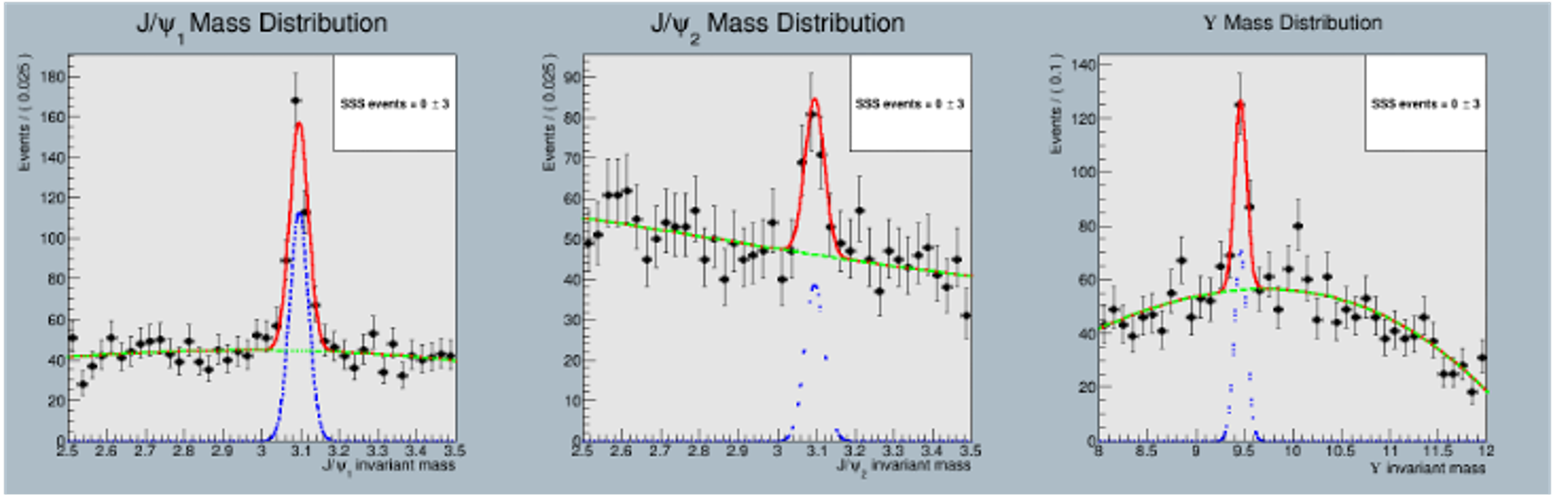
\includegraphics[width=1.0\linewidth]{images/JpsiJpsiY_fit.png}
    \caption{Fit result projection on individual invariant mass spectra}
    \label{fig:JpsiJpsiY_fit}
\end{figure}

The fit result projection is shown in Figure  \ref{fig:JpsiJpsiY_fit}, with no significant results.

\begin{table}[]
    \centering
    \caption{}
    \begin{tabular}{cc}
        \toprule
        \textbf{Yield Parameter} & \textbf{Value} \\
        \midrule
        $N(J/\psi^{[1], \text{sig} },J/\psi^{[2],\text{sig} }, \Upsilon^\text{sig})$ & $0 \pm 3$ \\
        $N(J/\psi^{[1], \text{bkg} },J/\psi^{[2],\text{sig} }, \Upsilon^\text{sig})$ & $7 \pm 7$ \\
        $N(J/\psi^{[1], \text{sig} },J/\psi^{[2],\text{bkg} }, \Upsilon^\text{sig})$ & $1 \pm 9$ \\
        $N(J/\psi^{[1], \text{sig} },J/\psi^{[2],\text{sig} }, \Upsilon^\text{bkg})$ & $9 \pm 8$ \\
        $N(J/\psi^{[1], \text{bkg} },J/\psi^{[2],\text{bkg} }, \Upsilon^\text{sig})$ & $102 \pm 19$ \\
        $N(J/\psi^{[1], \text{bkg} },J/\psi^{[2],\text{sig} }, \Upsilon^\text{bkg})$ & $80 \pm 19$ \\
        $N(J/\psi^{[1], \text{sig} },J/\psi^{[2],\text{bkg} }, \Upsilon^\text{bkg})$ & $263 \pm 25$ \\
        $N(J/\psi^{[1], \text{bkg} },J/\psi^{[2],\text{bkg} }, \Upsilon^\text{bkg})$ & $1544 \pm 48$ \\
        \bottomrule
    \end{tabular}
    \label{tab:my_label}
\end{table}

The predominant background seen from fitting is the double-$J/\psi$ events without $\Upsilon$ mesons. The low yield is believed to be due to the low cross section of the process.

\subsubsection{Estimation of $\sigma_{\text{TPS}}^{pp\to J/\psi+J/\psi+\Upsilon+X}$}

For the TPS component of the $pp\to J/\psi+J/\psi+\Upsilon+X$ process, the TPS effective cross section is taken to be $\effXsecTPS \approx 3 ~\text{mb}$ for this estimation. With SPS cross section reference values shown in Table \ref{tab:sps_xsec}, the TPS cross section is estimated to be:

\begin{equation}
    \begin{aligned}
    & \sigma_{\text{TPS}}^{pp\to J/\psi+J/\psi+\Upsilon+X} \times \mathfrak{B}_{J/\psi\to\mu\mu}^2\mathfrak{B}_{\Upsilon\to\mu\mu} \\
    & = \frac{2}{3!} \frac{\left(\sigma^{pp\to J/\psi+X}_{\text{SPS}}\right)^2\sigma^{pp\to \Upsilon+X}_{\text{SPS}}}{\effXsecTPS}\times \mathfrak{B}_{J/\psi\to\mu\mu}^2\mathfrak{B}_{\Upsilon\to\mu\mu} \\
    & = \frac{1}{3} \frac{\left(\sigma^{pp\to J/\psi+X}_{\text{SPS}}\times \mathfrak{B}_{J/\psi\to\mu\mu}\right)^2\left(\sigma^{pp\to \Upsilon+X}_{\text{SPS}}\times\mathfrak{B}_{\Upsilon\to\mu\mu}\right)}{\effXsecTPS} \\
    & \approx 0.36 ~\text{ab}
    \end{aligned} 
\end{equation}

At present statistics ($\mathcal{L} \approx 176.6 ~\text{fb}^{-1}$), we expect much less than 1 event for the TPS contribution and $\approx 1$ event with full Run 4 data ($\mathcal{L} \approx 3 ~\text{ab}^{-1}$), given present analysis strategy. A more efficient analysis strategy is needed to study this process.

\begin{table}[h!]
    \centering
    \caption{Caption}
    \begin{tabular}{p{0.2\linewidth} p{0.38\linewidth} p{0.35\linewidth}}
    \toprule
        Process & Fiducial Region & Estimated Cross-section \\
    \midrule
        \multirow{2}{\linewidth}{$pp\to J/\psi+X$}&
        $p_T\geq 6.0 \GeVc$ &
        \multirow{2}{\linewidth}{$\sigma(pp\to J/\psi+X) \times \mathfrak{B}_{J/\psi\to\mu\mu} \approx 80 ~\text{nb}$} \\
        & $|y| < 2.4$& \\
        \multirow{2}{\linewidth}{$pp\to \Upsilon(nS) +X$}&
        $p_T\in [10,120] \GeVc$ &
        \multirow{2}{\linewidth}{$\sigma(pp\to \Upsilon+X) \times \mathfrak{B}_{\Upsilon\to\mu\mu} \approx 1~\text{nb}$} \\
        & $|y| < 1.2$& \\
    \bottomrule
    \end{tabular}
    \label{tab:sps_xsec}
\end{table}

\section{Monte-Carlo (MC) Simulation Studies}

\subsection{Software Used for Monte Carlo Event Generation and Simulation}

HELAC-Onia 2.0 is an automated matrix element calculation tool dedicated to heavy-flavour quarkonia (such as $J/\psi$ and $\Upsilon(nS)$) studies. The matrix elements involved in heavy-flavour quarkonia production are calculated base on a NRQCD framework, giving the cross-section and dynamics characteristics in relevant processes and producing simulated events in Les Houches Event (LHE) format.\cite{HS_SHAO_HO}\cite{HS_SHAO_HO_2}

\textsc{Pythia 8} is a general-purpose event generator capable of simulating processes including hard scattering, parton showering, hadronization and decay in high-energy particle collisions.\cite{PYTHIA_8_2}

\textsc{Geant 4} is a toolkit for particle-detector interaction simulation, with the capability of simulating the motion and interaction of particles in complex detector geometry and simulate the interaction between particles and detector modules in the broad energy range from eV to TeV level.\cite{GEANT4}

CMS offline software (\textsc{CMSSW}) is a collection of software built for the CMS experiment, with the high-level goals of processing and selecting events inside the HLT system, delivering the processed results to the experimenters within the CMS Collaboration, and providing tools for them to analyze the processed data in order to produce physics results. The software employs a general data format of Event Data Model (EDM) and provides the services needed by the simulation, calibration and alignment, and reconstruction modules that process event data for physics analysis.\cite{CMS_PHYS_TDR}

\subsection{MC Simulation Procedure Based on \textsc{CMSSW}}\label{sec:MC-FullChain}

\subsubsection{"GEN-SIM" Steps}

This analysis uses \textsc{HELAC-Onia 2.7.6} to generate event samples of $pp\to J/\psi+J/\psi+\Upsilon(1S)+X$ in proton collisions, and stores the initial particle information in LHE file format. Subsequently, \textsc{Pythia 8} is used to simulate the decay of $J/\psi$ and $\Upsilon$, as well as the hadronization processes of other particles, yielding information on the  energies, momenta, and decay vertices of particles interacting with the detector, which is stored as GEN format data.

Based on this information, \textsc{Geant 4} is used to model the interactions of generated particles with the various detector units in the CMS detector, taking into account the magnetic field and overall geometric configuration, and output GENSIM format data containing particle properties and detector responses.

\subsubsection{"DIGI-RAW-MIX" Steps}

Starting from the GENSIM format data, the digitization process in which the detector responses are converted into digital signals is performed, simulating the response of the CMS detector to the generated particles. Event samples simulating the pileup effect are obtained from a "MinBias premix dataset" and overlapped onto the simulated events. RAWSIM format data is then generated, which contains the digitized signals from the detector, including the effects of pileup.

\subsubsection{"RECO-SKIM" Steps}

Starting from the RAWSIM format, the L1T and HLT processes are further simulated, filtering events and outputting raw data (RAW); Subsequently, particle tracks and jets are reconstructed, generating AODSIM (analysis object data simulation) format data, which retains simplified particle information. After further skimming, MINIAODSIM format data is formed and handed over to the previously developed analysis framework for further processing, ultimately completing the entire simulation analysis workflow.

\subsubsection{Computing Resources Used in MC Generation}

To improve overall data processing speed, we utilise the CMS collaboration's CRAB computing resources and data management system to submit computing tasks to CERN's computing grid, achieving a complete data processing workflow from LHE files to Ntuples. The relevant configuration file documentation has been compiled into a working document and uploaded to the GitHub repository \href{https://github.com/Eric100911/LHE-to-SKIM}{Eric100911/LHE-to-SKIM}.

\subsubsection{Event Mixing Method Employed in Event Generation}

The simulation generation methods for $pp\to J/\psi+J/\psi+\Upsilon(1S)+X$ events generated by different mechanisms are also different. With the pp\_NOnia\_MPS plugin in HELAC-Onia 2.7.6, TPS events of $pp\to J/\psi+J/\psi+\Upsilon(1S)+X$ are directly obtained. For the DPS process, it is necessary to first generate samples of $J/\psi+J/\psi$ and $J/\psi+\Upsilon$ produced through SPS process, as well as single-$J/\psi$ and single-$\Upsilon$ produced. Based on this, by performing random mixing, two types of simulated samples of $J/\psi+J/\psi+\Upsilon$ produced by the DPS process.

\subsection{LHE-level $pp\to J/\psi+J/\psi+\Upsilon+X$ Event Simulation Studies}

\subsubsection{Event Generation and Filtering}

A series of event samples was generated using HELAC-Onia 2.7.6, with generator-level filter shown in Table \ref{tab:JpsiJpsiY_MC_GEN_Filter}. 

\begin{table}[]
    \centering
    \caption{Generation-level Event Filter Criteria for $pp\to J/\psi+J/\psi+\Upsilon+X$\\}
    \label{tab:JpsiJpsiY_MC_GEN_Filter}
    \begin{tabular}{cc}
        \toprule
        \textbf{Object} & \textbf{Criteria} \\
        \midrule
        Generated $J/\psi $     &   $\left|y\right|<2.5$ \\
                                &   $p_T > 2.0\GeVc$ \\
        Generated $\Upsilon(1S)$&   $\left|y\right|<2.5$ \\
                                &   $p_T > 2.0\GeVc$ \\
        \bottomrule
    \end{tabular}
\end{table}

A sample of 112885 $pp\to J/\psi+J/\psi+\Upsilon(1S)+X$ events was generated without filtering, with the following components:

\begin{itemize}
    \item 100000 TPS events of $pp\to J/\psi+J/\psi+\Upsilon(1S)+X$;
    \item 4279 DPS events of $pp\to J/\psi+J/\psi+\Upsilon(1S)+X$, with one $J/\psi$ and one $\Upsilon(1S)$ produced in the same sub-scattering ("DPS-01");
    \item 8606 DPS events of $pp\to J/\psi+J/\psi+\Upsilon(1S)+X$, with two $J/\psi$ produced in the same sub-scattering ("DPS-02");
\end{itemize}

After applying the generator-level filter (Table \ref{tab:JpsiJpsiY_MC_GEN_Filter}), a total of 4772 events were obtained, with the following components:

\begin{itemize}
    \item 4455 TPS events of $pp\to J/\psi+J/\psi+\Upsilon(1S)+X$;
    \item 132 DPS events of $pp\to J/\psi+J/\psi+\Upsilon(1S)+X$, with one $J/\psi$ and one $\Upsilon(1S)$ produced in the same sub-scattering ("DPS-01");
    \item 185 DPS events of $pp\to J/\psi+J/\psi+\Upsilon(1S)+X$, with two $J/\psi$ produced in the same sub-scattering ("DPS-02");
\end{itemize}

These filtered event samples, stored in Les Houches Event (LHE) format, are used for further analysis in the following sections.

\subsubsection{Demonstrating Particle Correlation at LHE Level with $\Delta y - \Delta \phi$ Distribution Plot}

The correlation between the produced particles can be demonstrated through the $\Delta y - \Delta \phi$ and $\Delta |y| - \Delta \phi$ distribution of the generated particles. At LHE level, the distribution is presented in Figures \ref{fig:TPS_JJY1S_filtered_correlation_LHE}, \ref{fig:DPS01_JJY1S_filtered_correlation_LHE} and \ref{fig:DPS02_JJY1S_filtered_correlation_LHE}.

\begin{figure}
    \centering
    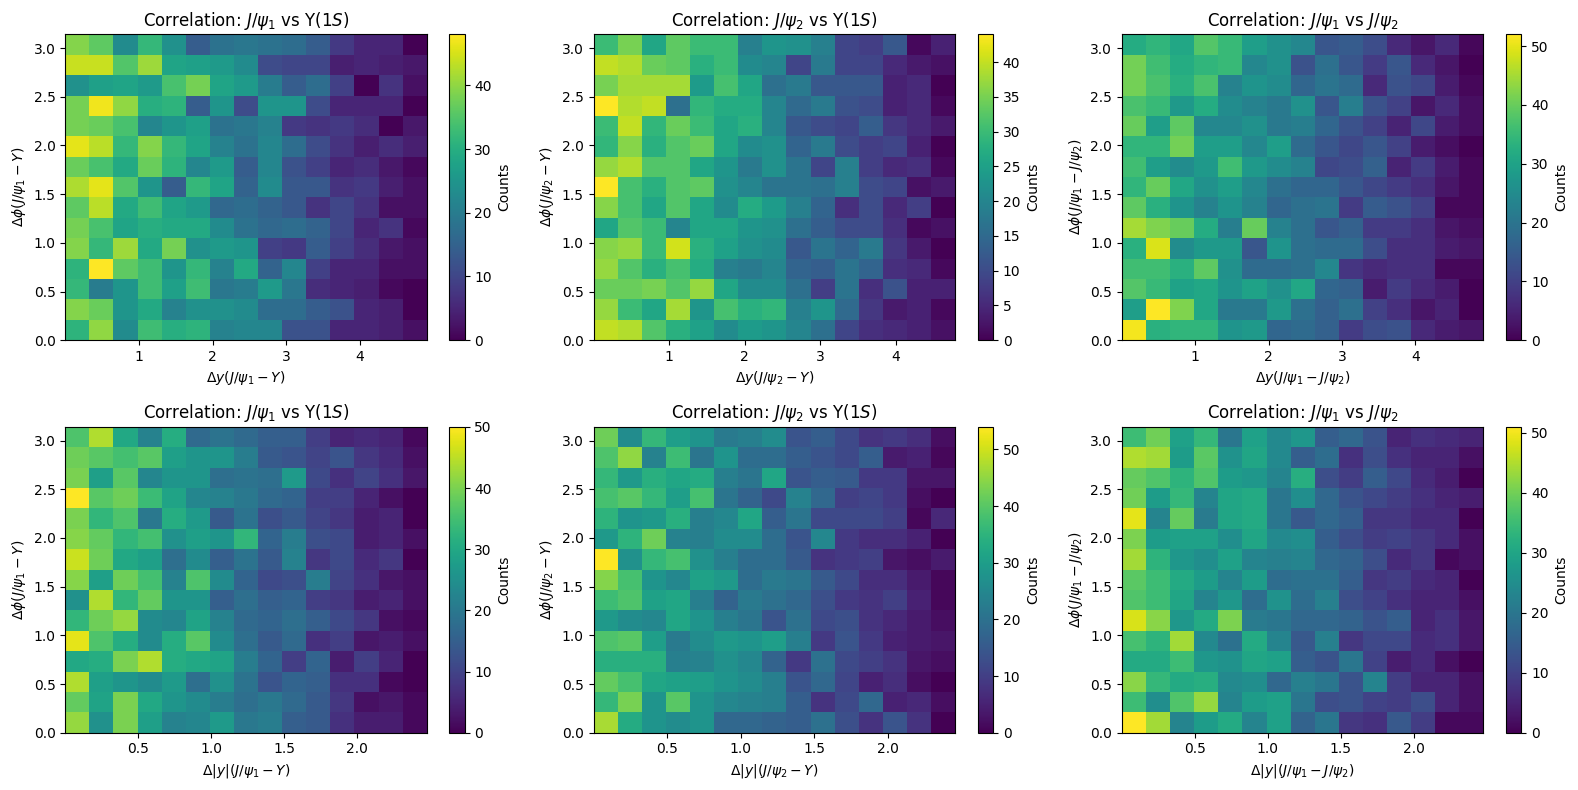
\includegraphics[width=1.0\linewidth]{images/yabs_LHE_LEVEL_TPS_JJY1S_correlation_filtered_p2.png}
    \caption{Correlation between generated particles in TPS $pp\to J/\psi+J/\psi+\Upsilon(1S)+X$ events at LHE level}
    \label{fig:TPS_JJY1S_filtered_correlation_LHE}
\end{figure}

\begin{figure}
    \centering
    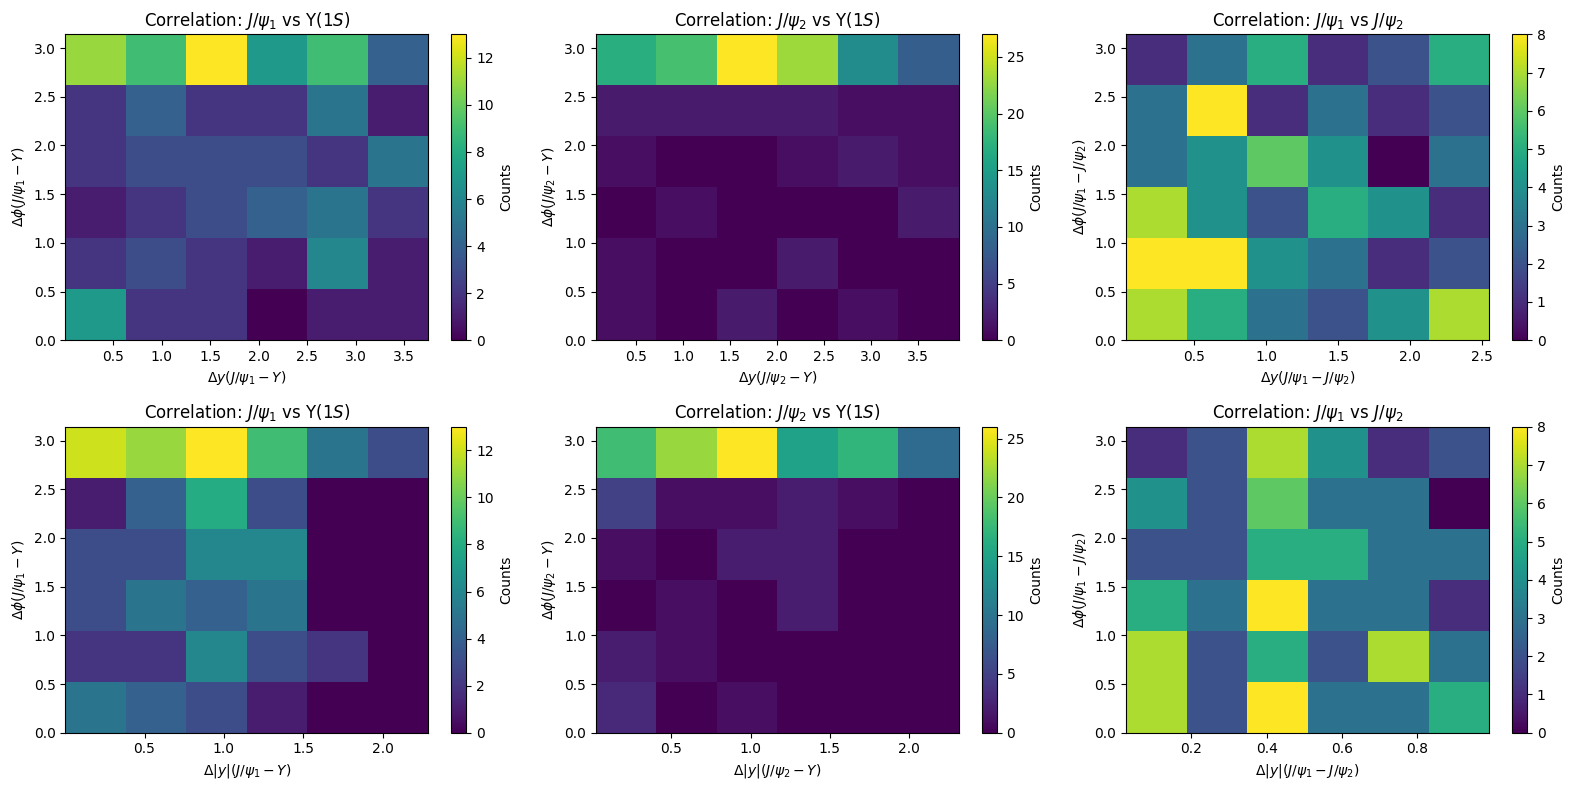
\includegraphics[width=1.0\linewidth]{images/yabs_LHE_LEVEL_DPS_JY1S_J_correlation_filtered_p2.png}
    \caption{Correlation between generated particles in DPS-01 $pp\to J/\psi+J/\psi+\Upsilon(1S)+X$ events at LHE level}
    \label{fig:TPS_JJY1S_filtered_correlation_LHE}
\end{figure}

\begin{figure}
    \centering
    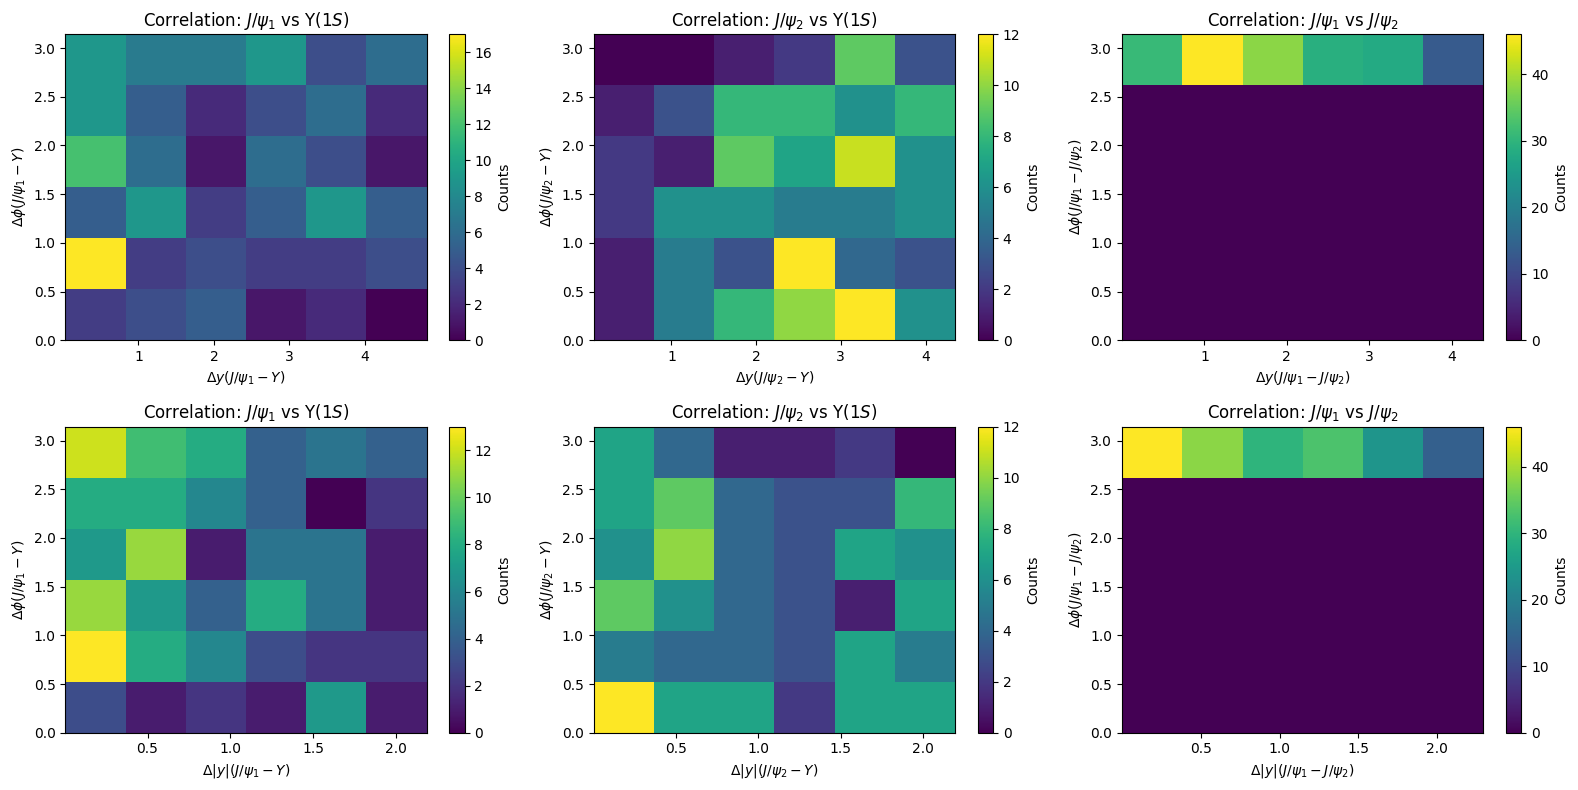
\includegraphics[width=1.0\linewidth]{images/yabs_LHE_LEVEL_DPS_JJ_Y1S_correlation_filtered_p2.png}
    \caption{Correlation between generated particles in DPS-02 $pp\to J/\psi+J/\psi+\Upsilon(1S)+X$ events at LHE level}
    \label{fig:TPS_JJY1S_filtered_correlation_LHE}
\end{figure}

The difference in the correlation between the generated particles in TPS and DPS processes is evident, especially in the $\Delta \phi$ projection. These plots demonstrate the feasibility of separating the components in the subsequent analysis. Such properties can also be seen on the one dimensional distribution of $\Delta y$, $\Delta \phi$ and $\Delta R$ in Figures .

\begin{figure}
    \centering
    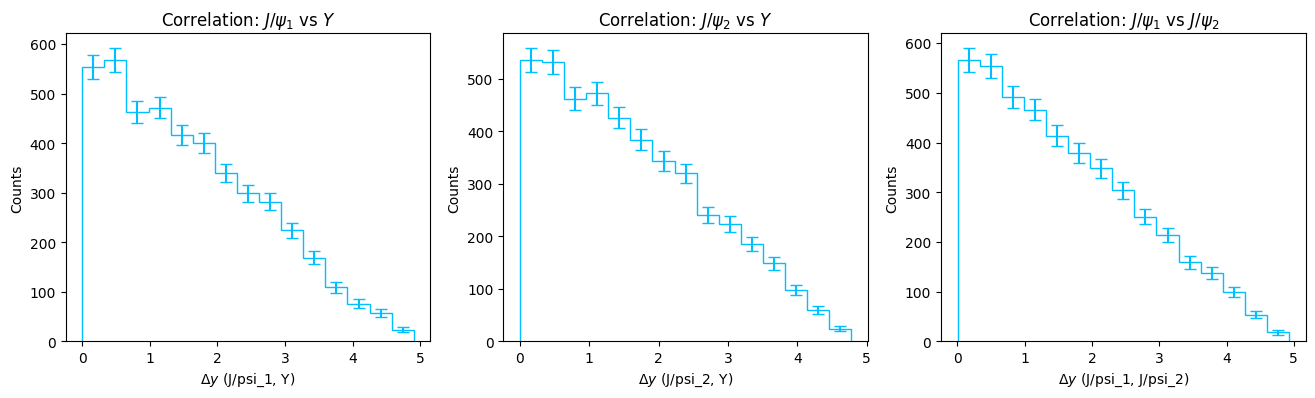
\includegraphics[width=1.0\linewidth]{images/LHE_LEVEL_TPS_DeltaY_filtered.png}
    \caption{Distribution of $\Delta y$ in TPS $pp\to J/\psi+J/\psi+\Upsilon(1S)+X$ events passing filter condition in Table \ref{tab:JpsiJpsiY_MC_GEN_Filter} at LHE level}
    \label{fig:TPS_JJY1S_filtered_DeltaY_LHE}
\end{figure}

\begin{figure}
    \centering
    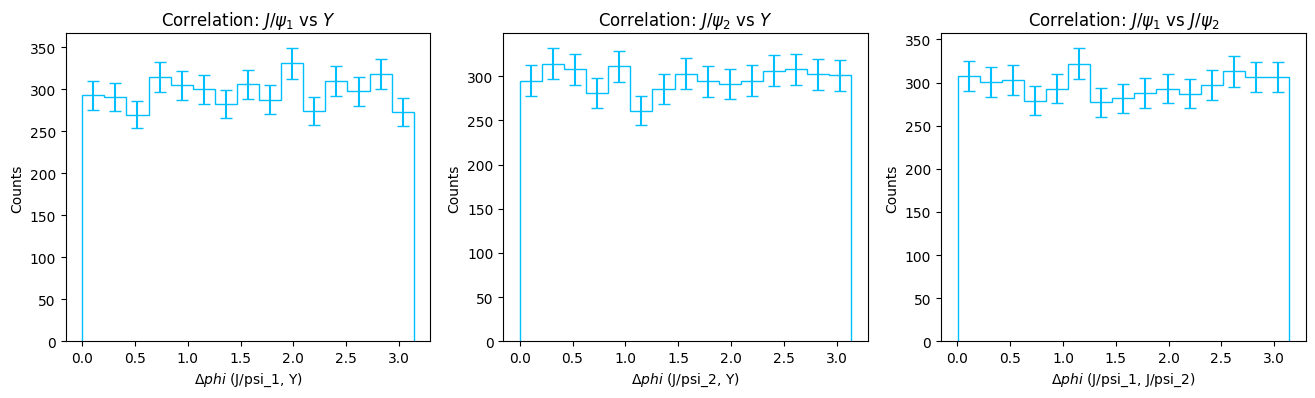
\includegraphics[width=1.0\linewidth]{images/LHE_LEVEL_TPS_DeltaPhi_filtered.png}
    \caption{Distribution of $\Delta \phi$ in TPS $pp\to J/\psi+J/\psi+\Upsilon(1S)+X$ events passing filter condition in Table \ref{tab:JpsiJpsiY_MC_GEN_Filter} at LHE level}
    \label{fig:TPS_JJY1S_filtered_DeltaPhi_LHE}
\end{figure}

\begin{figure}
    \centering
    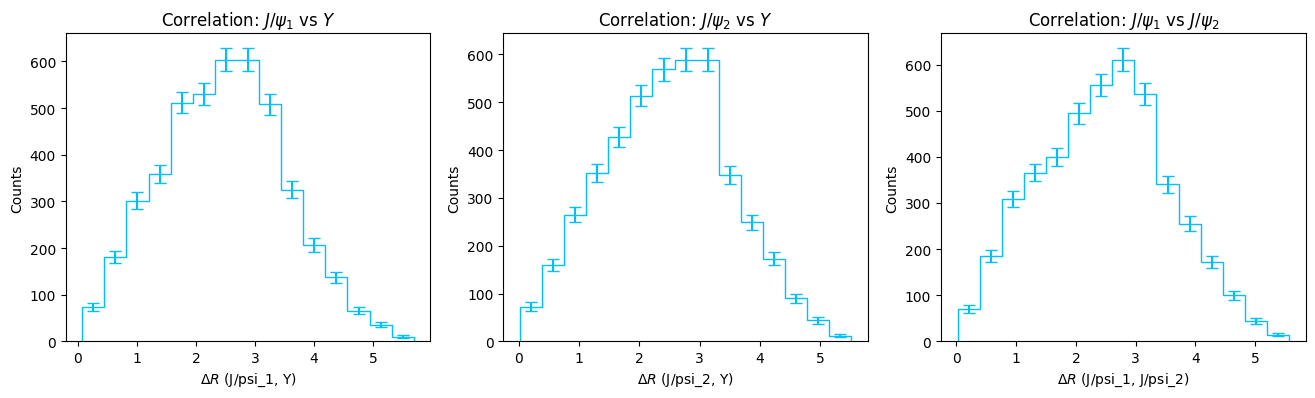
\includegraphics[width=1.0\linewidth]{images/LHE_LEVEL_TPS_DeltaR_filtered.png}
    \caption{Distribution of $\Delta R$ in TPS $pp\to J/\psi+J/\psi+\Upsilon(1S)+X$ events passing filter condition in Table \ref{tab:JpsiJpsiY_MC_GEN_Filter} at LHE level}
    \label{fig:TPS_JJY1S_filtered_DeltaR_LHE}
\end{figure}

\begin{figure}
    \centering
    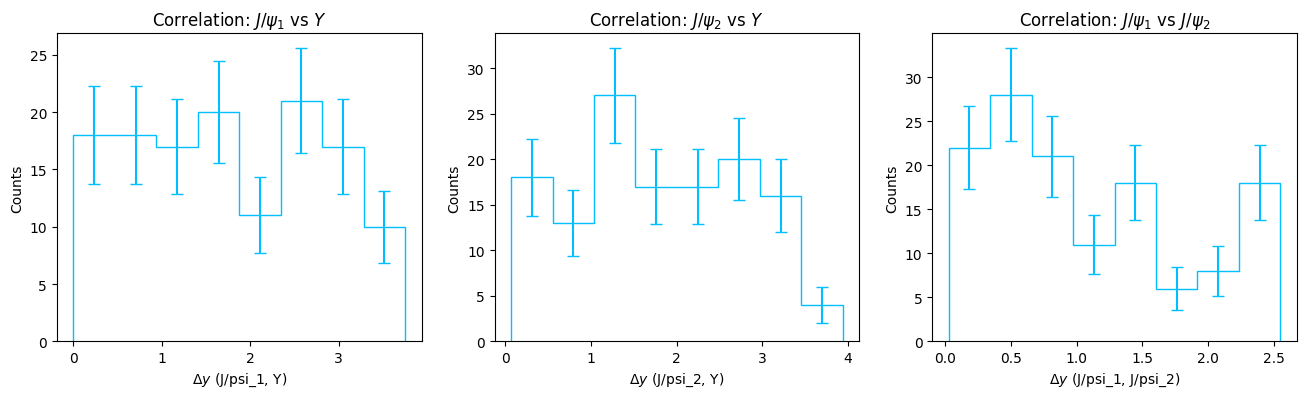
\includegraphics[width=1.0\linewidth]{images/LHE_LEVEL_DPS_J_JY1S_DeltaY_filtered.png}
    \caption{Distribution of $\Delta y$ in DPS-01 $pp\to J/\psi+J/\psi+\Upsilon(1S)+X$ events passing filter condition in Table \ref{tab:JpsiJpsiY_MC_GEN_Filter} at LHE level}
    \label{fig:DPS01_JJY1S_filtered_DeltaY_LHE}
\end{figure}

\begin{figure}
    \centering
    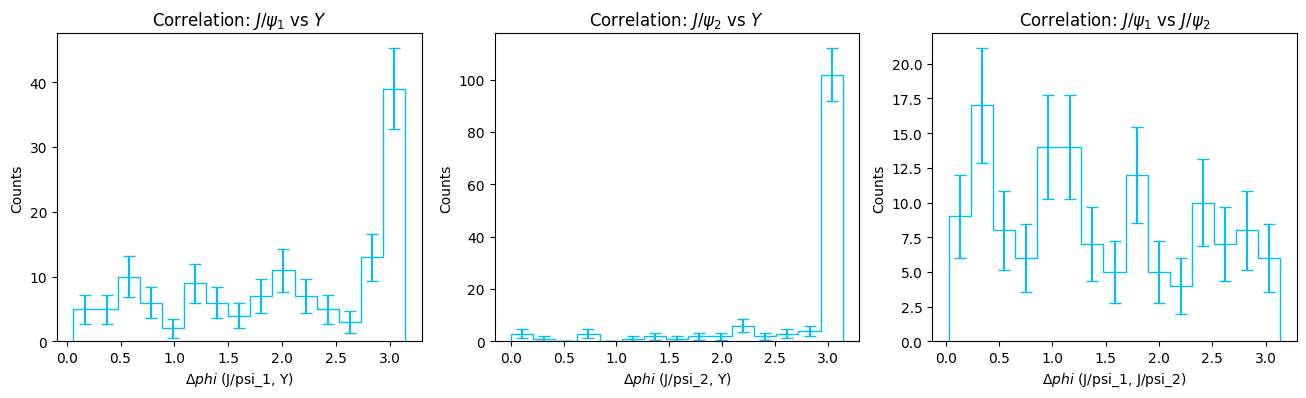
\includegraphics[width=1.0\linewidth]{images/LHE_LEVEL_DPS_J_JY1S_DeltaPhi_filtered.png}
    \caption{Distribution of $\Delta \phi$ in DPS-01 $pp\to J/\psi+J/\psi+\Upsilon(1S)+X$ events passing filter condition in Table \ref{tab:JpsiJpsiY_MC_GEN_Filter} at LHE level}
    \label{fig:DPS01_JJY1S_filtered_DeltaPhi_LHE}
\end{figure}

\begin{figure}
    \centering
    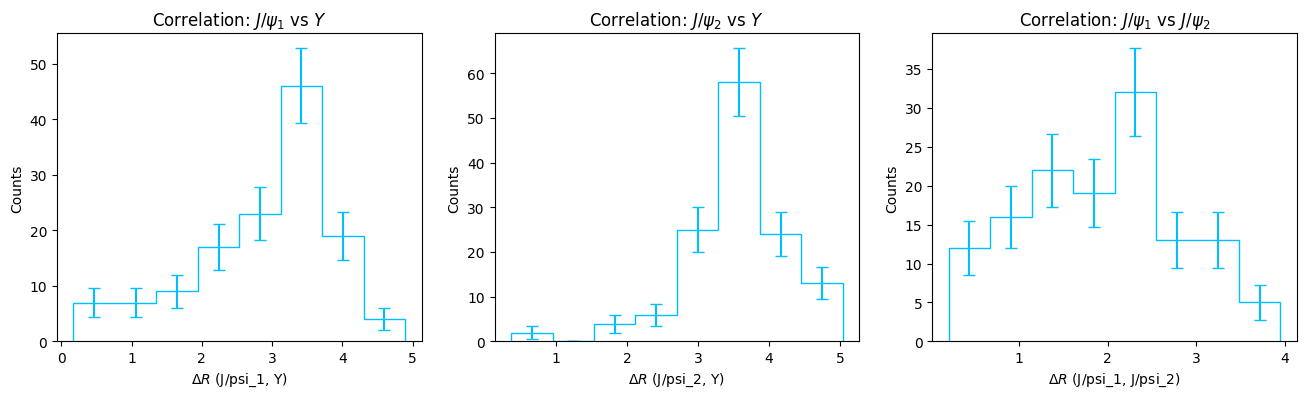
\includegraphics[width=1.0\linewidth]{images/LHE_LEVEL_DPS_J_JY1S_DeltaR_filtered.png}
    \caption{Distribution of $\Delta R$ in DPS-01 $pp\to J/\psi+J/\psi+\Upsilon(1S)+X$ events passing filter condition in Table \ref{tab:JpsiJpsiY_MC_GEN_Filter} at LHE level}
    \label{fig:DPS01_JJY1S_filtered_DeltaR_LHE}
\end{figure}

\begin{figure}
    \centering
    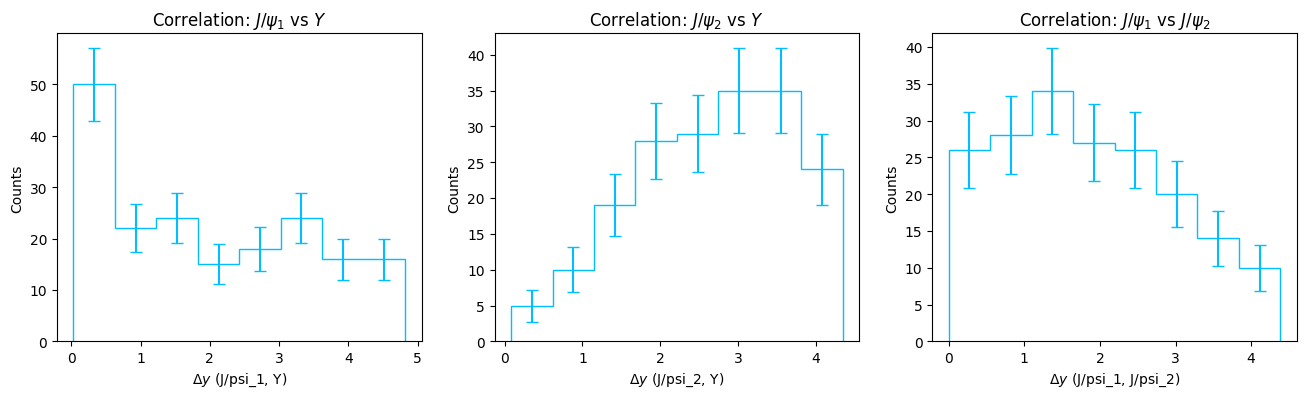
\includegraphics[width=1.0\linewidth]{images/LHE_LEVEL_DPS_JJ_Y1S_DeltaY_filtered.png}
    \caption{Distribution of $\Delta y$ in DPS-02 $pp\to J/\psi+J/\psi+\Upsilon(1S)+X$ events passing filter condition in Table \ref{tab:JpsiJpsiY_MC_GEN_Filter} at LHE level}
    \label{fig:DPS02_JJY1S_filtered_DeltaY_LHE}
\end{figure}

\begin{figure}
    \centering
    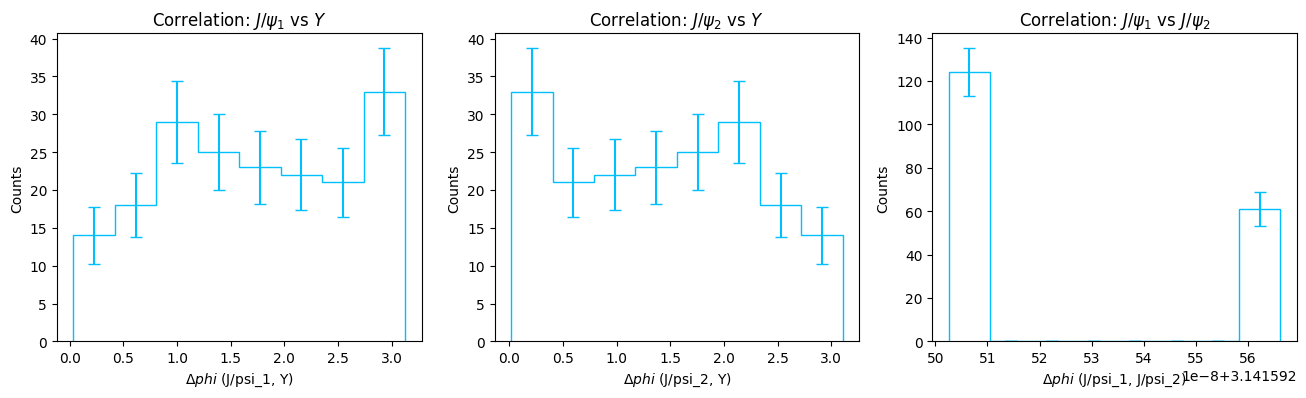
\includegraphics[width=1.0\linewidth]{images/LHE_LEVEL_DPS_JJ_Y1S_DeltaPhi_filtered.png}
    \caption{Distribution of $\Delta \phi$ in DPS-02 $pp\to J/\psi+J/\psi+\Upsilon(1S)+X$ events passing filter condition in Table \ref{tab:JpsiJpsiY_MC_GEN_Filter} at LHE level}
    \label{fig:DPS02_JJY1S_filtered_DeltaPhi_LHE}
\end{figure}

\begin{figure}
    \centering
    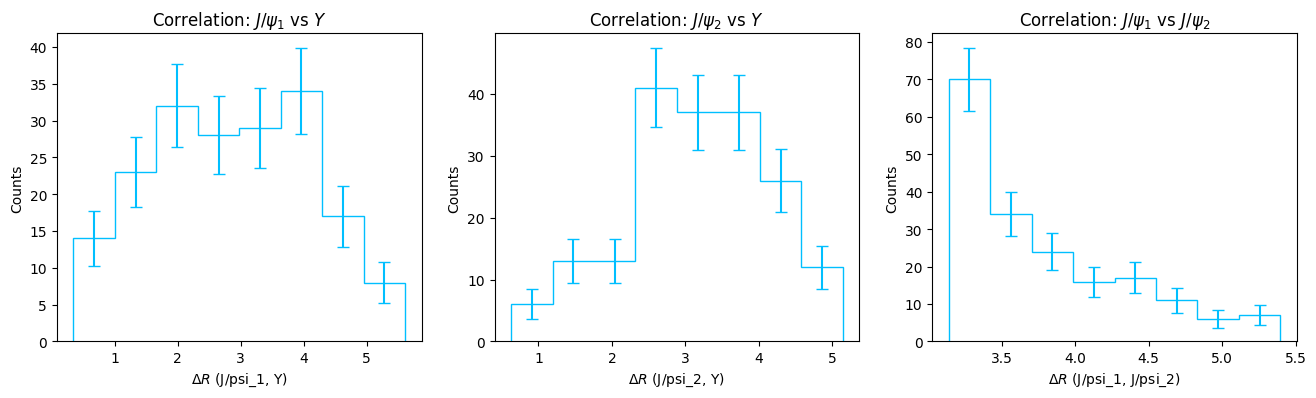
\includegraphics[width=1.0\linewidth]{images/LHE_LEVEL_DPS_JJ_Y1S_DeltaR_filtered.png}
    \caption{Distribution of $\Delta R$ in DPS-02 $pp\to J/\psi+J/\psi+\Upsilon(1S)+X$ events passing filter condition in Table \ref{tab:JpsiJpsiY_MC_GEN_Filter} at LHE level}
    \label{fig:DPS02_JJY1S_filtered_DeltaR_LHE}
\end{figure}

The LHE-level results show the feasibility of separating DPS and TPS components by the $\Delta \phi$, $\Delta R$ and $\Delta y - \Delta \phi$ correlation plots.

To gain a more realistic prediction of particle correlation, a set of full-chain simulation and reconstruction is performed as the procedure described in the section \ref{sec:MC-FullChain}. Simulation results are presented in the next section.

\subsection{Full-chain $pp\to J/\psi+J/\psi+\Upsilon+X$ Event Simulation Results}

A sample of approximately $3.6\times 10^6$ TPS $pp\to J/\psi+J/\psi+\Upsilon(1S)+X$ events was generated using HELAC-Onia 2.7.6, without any generator-level filter. The events were then processed through the full chain of simulation and reconstruction described in Section \ref{sec:MC-FullChain}. After passing the full filter condition shown in Table \ref{tab:JpsiJpsiY_MC_Full_Filter}, a total of 441 events were obtained. Due to limited statistics, only individual $\Delta \phi$, $\Delta y$ and $\Delta R$ distributions are plotted. 

\begin{table}[]
    \centering
    \caption{Full-chain Event Selection Criteria for $pp\to J/\psi+J/\psi+\Upsilon(1S)+X$\\}
    \begin{tabular}{p{0.25\linewidth} p{0.65\linewidth}}
    \toprule
        \textbf{Object} & \textbf{Criteria} \\
        Generated $J/\psi $         & $\left|y\right|<3$ \\
        \midrule
        Generated $\Upsilon(1S)$    & $\left|y\right|<3$ \\
        \midrule
        Reconstructed $\mu^\pm $ & Muon ID "soft" \\
                & $|\eta| < 2.4$ \\
                & $p_T > 3.5\GeVc$ for $|\eta| < 1.2$ \\
                & $p_T > 2.5\GeVc$ for $1.2 < |\eta| < 2.4$ \\
        Reconstructed Charged Tracks & High Purity \\
                  & $|\eta|<2.5$ \\
                  & $p_T > 2.0 \GeVc$ \\
        \midrule
        Reconstructed $J/\psi$ & $2.9 \GeVcs < m_{\mu\mu} < 3.3 \GeVcs$ \\
                & $p_T > 4.0\GeVc$ \\
                & $|y| < 2.5$ \\
                & Opposite-sign muon pairs fitted to common vertex with $> 0.5\%$ probability \\
        \midrule
        Reconstructed $\Upsilon(1S)$ & $8.5\GeVcs < m_{\mu\mu} < 11.4 \GeVcs$ \\
                & $p_T > 4.0\GeVc$ \\
                & $|y| < 2.5$ \\
                & Opposite-sign muon pairs fitted to common vertex with $> 0.5\%$ probability \\
        \bottomrule
    \end{tabular}
    \label{tab:JpsiJpsiY_MC_Full_Filter}
\end{table}

\begin{figure}
    \centering
    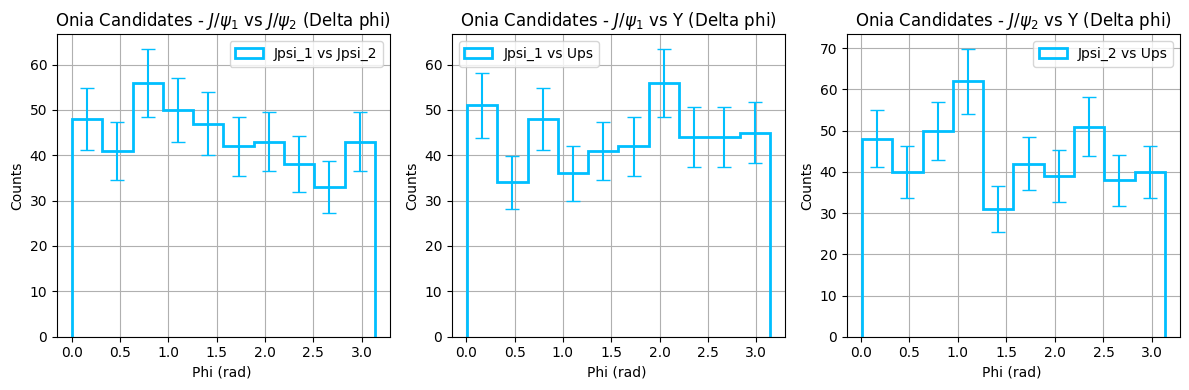
\includegraphics[width=1.0\linewidth]{images/Ntuple_LEVEL_TPS_DeltaPhi_filtered.png}
    \caption{Distribution of $\Delta \phi$ in TPS $pp\to J/\psi+J/\psi+\Upsilon(1S)+X$ events passing filter condition in Table \ref{tab:JpsiJpsiY_MC_Full_Filter} after complete simulation and reconstruction}
    \label{fig:TPS_JJY1S_filtered_DeltaPhi_Ntuple}
\end{figure}

\begin{figure}
    \centering
    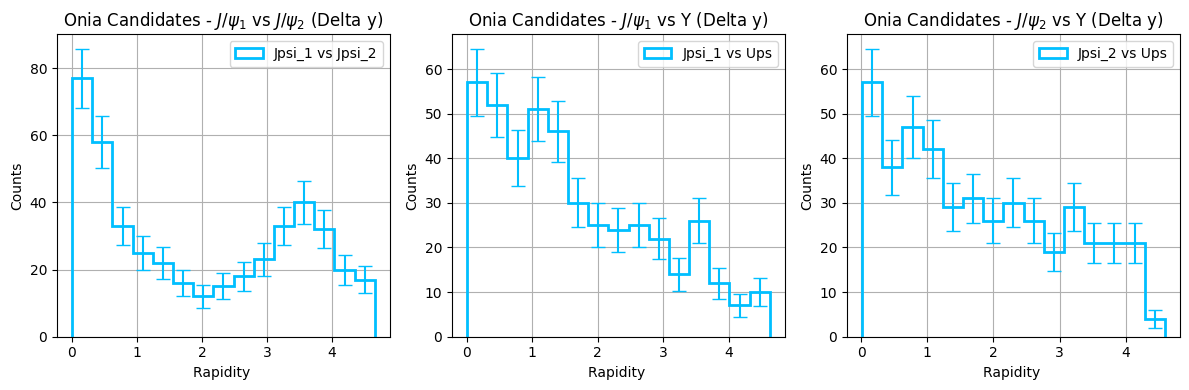
\includegraphics[width=1.0\linewidth]{images/Ntuple_LEVEL_TPS_DeltaY_filtered.png}
    \caption{Distribution of $\Delta y$ in TPS $pp\to J/\psi+J/\psi+\Upsilon(1S)+X$ events passing filter condition in Table \ref{tab:JpsiJpsiY_MC_Full_Filter} after complete simulation and reconstruction}
    \label{fig:TPS_JJY1S_filtered_DeltaY_Ntuple}
\end{figure}

\begin{figure}
    \centering
    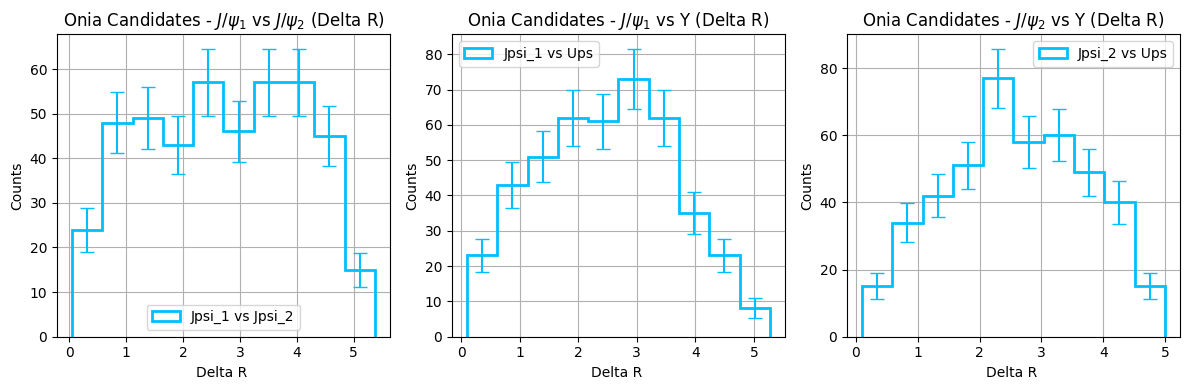
\includegraphics[width=1.0\linewidth]{images/Ntuple_LEVEL_TPS_DeltaR_filtered.png}
    \caption{Distribution of $\Delta R$ in TPS $pp\to J/\psi+J/\psi+\Upsilon(1S)+X$ events passing filter condition in Table \ref{tab:JpsiJpsiY_MC_Full_Filter} after complete simulation and reconstruction}
    \label{fig:TPS_JJY1S_filtered_DeltaR_Ntuple}
\end{figure}

An unusual result can be seen in the $\Delta y (J/\psi_1, J/\psi_2)$ distribution (Figure \ref{fig:TPS_JJY1S_filtered_DeltaY_Ntuple}) when compared to the LHE-level result in Figure \ref{fig:TPS_JJY1S_filtered_DeltaY_LHE}, where a significant lump is seen at $\Delta y \approx 3.5$. This may be due to detector efficiency effects or a some error from the simulation chain. Further investigation is needed to understand the cause of this anomaly.

\section{Conclusions}

\subsection{Collision Data Analysis Result Summary}

An analysis framework has developed for extracting $pp \to J/\psi+J/\psi+\phi+X$, $pp \to J/\psi+J/\psi+\Upsilon+X$ and $pp \to J/\psi+J/\psi+\Upsilon+X$ processes from the Run 3 data of the CMS experiment. Evidence has been found for $pp \to J/\psi+J/\psi+\phi+X$ process with a signal significance of $4.7\sigma$ and $pp \to J/\psi+\Upsilon+\phi+X$ process with a signal significance of $2.98\sigma$. No clear evidence for $pp \to J/\psi+J/\psi+\Upsilon+X$ process has been found, which is believed as an result of a relatively low cross-section.

\subsection{Monte Carlo Simulation Result Summary}

A full-chain simulation and reconstruction framework has been developed for the $pp \to J/\psi+J/\psi+\Upsilon(1S)+X$ process. The feasibility of separating the TPS and DPS components has been demonstrated at the LHE level, with a clear difference in $\Delta \phi$, $\Delta R$, and $\Delta y - \Delta \phi$ correlation plots. The full-chain simulation results show a similar trend, but with some anomalies in the $\Delta y$ distribution that require further investigation.

\subsection{Further Work and Future Prospects}

In the upcoming months, an event generation framework for $pp\to J/\psi+J/\psi+\phi+X$ and $pp\to J/\psi+\Upsilon+\phi+X$ processes will be developed. More samples will be generated to improve the statistics of the analysis. A filter configuration will be introduced at generation-level to improve the overall efficiency of event generation and simulation.

With Monte Carlo samples, efficiency and systematic errors will be evaluated for the searched processes and can be used to determine the actual cross-section of the processes, employing event-by-event correction. Separation of the SPS, DPS and TPS components will also be studied in detail, with the aim of obtaining a more accurate estimation of the cross-section of the TPS component.

Most of the results above have been presented at the CMS B-physics Group Production and Properties Meeting on 9th July, 2025 by the author. Positive response has been received from the group members and the author would like to communicate with the primary author of the triple-$J/\psi$ study for further collaboration and discussion.

\subsection{Acknowledgements}

This work is carried out under the supervision of Dr. Zhen Hu and in collaboration with Xing Cheng from Zhili College and Zhenpeng Shi from Department of Physics.

Much help has been received from the Tsinghua CMS group, including but not limited to the following members: Dr. Zhen Hu, Yiyang Zhao, Xining Wang, Shiyang Chen. The author would like to express his gratitude for their help and support.

\bibliographystyle{abbrv}
\bibliography{refs}
\end{document}
